


\section{Amplification de l'effet photoelectrique par le chlore}

\subsection{Neufeld and Wolfire}

Les réseaux d'astrochimie de PDR ont tendance à négliger le chlore qui a une abondance mineure dans les nuages (voir \autoref{tab:gaz}). Or des espèces dérivées du chlore ont été observées en absorption dans des nuages diffus ($n \sim 10^2\ cm^{-3}$). Des raies de $\mathrm{H}_2\mathrm{Cl}^+$,HCl et $\mathrm{HCl}^+$ excitées ont également été observées par Herschel dans plusieurs sources de la Galaxie et notamment dans le nuage moléculaire de la barre d'Orion \cite{Neufeld2012,Neufire2009}. J'ai ajouté le réseau chimique du chlore dans le modèle PDR afin d'interpréter ces résultats. \newline

\subsection{Analyse du rôle du chlore}

\begin{figure}[htbp]
    \centering
    \begin{subfigure}[t]{0.45\textwidth} % "0.45" donne ici la largeur de l'image
        \centering \includegraphics[trim = {0 0 0 1cm},clip,width=1\textwidth]{figure/model_Cl/PDR155_n_d1e5r1e4A2e1.png}
        \caption{Profil de température et densité en fonction de la profondeur dans le nuage}\label{fig:ClT}
    \end{subfigure}
    ~ 
    \begin{subfigure}[t]{0.45\textwidth}
        \centering \includegraphics[trim = {0 0 0 1cm},clip,width=1\textwidth]{figure/model_Cl/tb_PDR155_n_d1e5r1e4A2e1.png}
        \caption{Taux de chauffage et refroidissement en fonction de la température du gaz au bord atomique du nuage ($A_{\mathrm{V}} = 10^{-6}$)}\label{fig:ClHC}
    \end{subfigure}
    \caption{Profil de densité de l'hydrogène et de la température en fonction de l'extinction dans le visible.}
\end{figure}

J'ai étudié les réactions chimiques principales qui se déroulent en bord de nuage atomique et démontré que le chlore joue le rôle de catalyseur de l'effet photoélectrique. Le mécanisme est illustré sur la \autoref{fig:catalyseur}.
Le champs de rayonnement UV, intense en bord de nuage atomique, photoionise le chlore et produit des ions $\mathrm{Cl}^+$ et des électrons. Le transfert de charge du $\mathrm{Cl}^+$ avec l'hydrogène est une réaction rapide qui permet au chlore de se rendre de nouveau disponible pour la photoionisation. Le chlore permet ainsi de ioniser indirectement l'hydrogène. Par conséquent, la fraction électronique du gaz augmente.  
Or on sait que l'effet photoélectrique sur les grains fonctionne d'autant plus que la fraction électronique dans le nuage est importante \footnote{Une forte densité d'électrons rend plus facile la recombinaison électronique des grains ce qui maintient le degré d'ionisation des grains raisonnablement faible. Il est plus facile d'arracher un électron d'un grain neutre que d'un grain qui a déjà été ionisé.}. 
L'effet photoélectrique chauffe ainsi le gaz ce qui améliore l'efficacité du transfert de charge du $\mathrm{Cl}^+$ avec l'hydrogène. 
En d'autres termes, le chlore induit une rétroaction positive de l'effet photoélectrique sur les grains. Cet emballement a tendance à chauffer le gaz à des températures nettement plus fortes et ce malgré la faible abondance du chlore. \newline

\begin{figure}[b!]
   \centering
        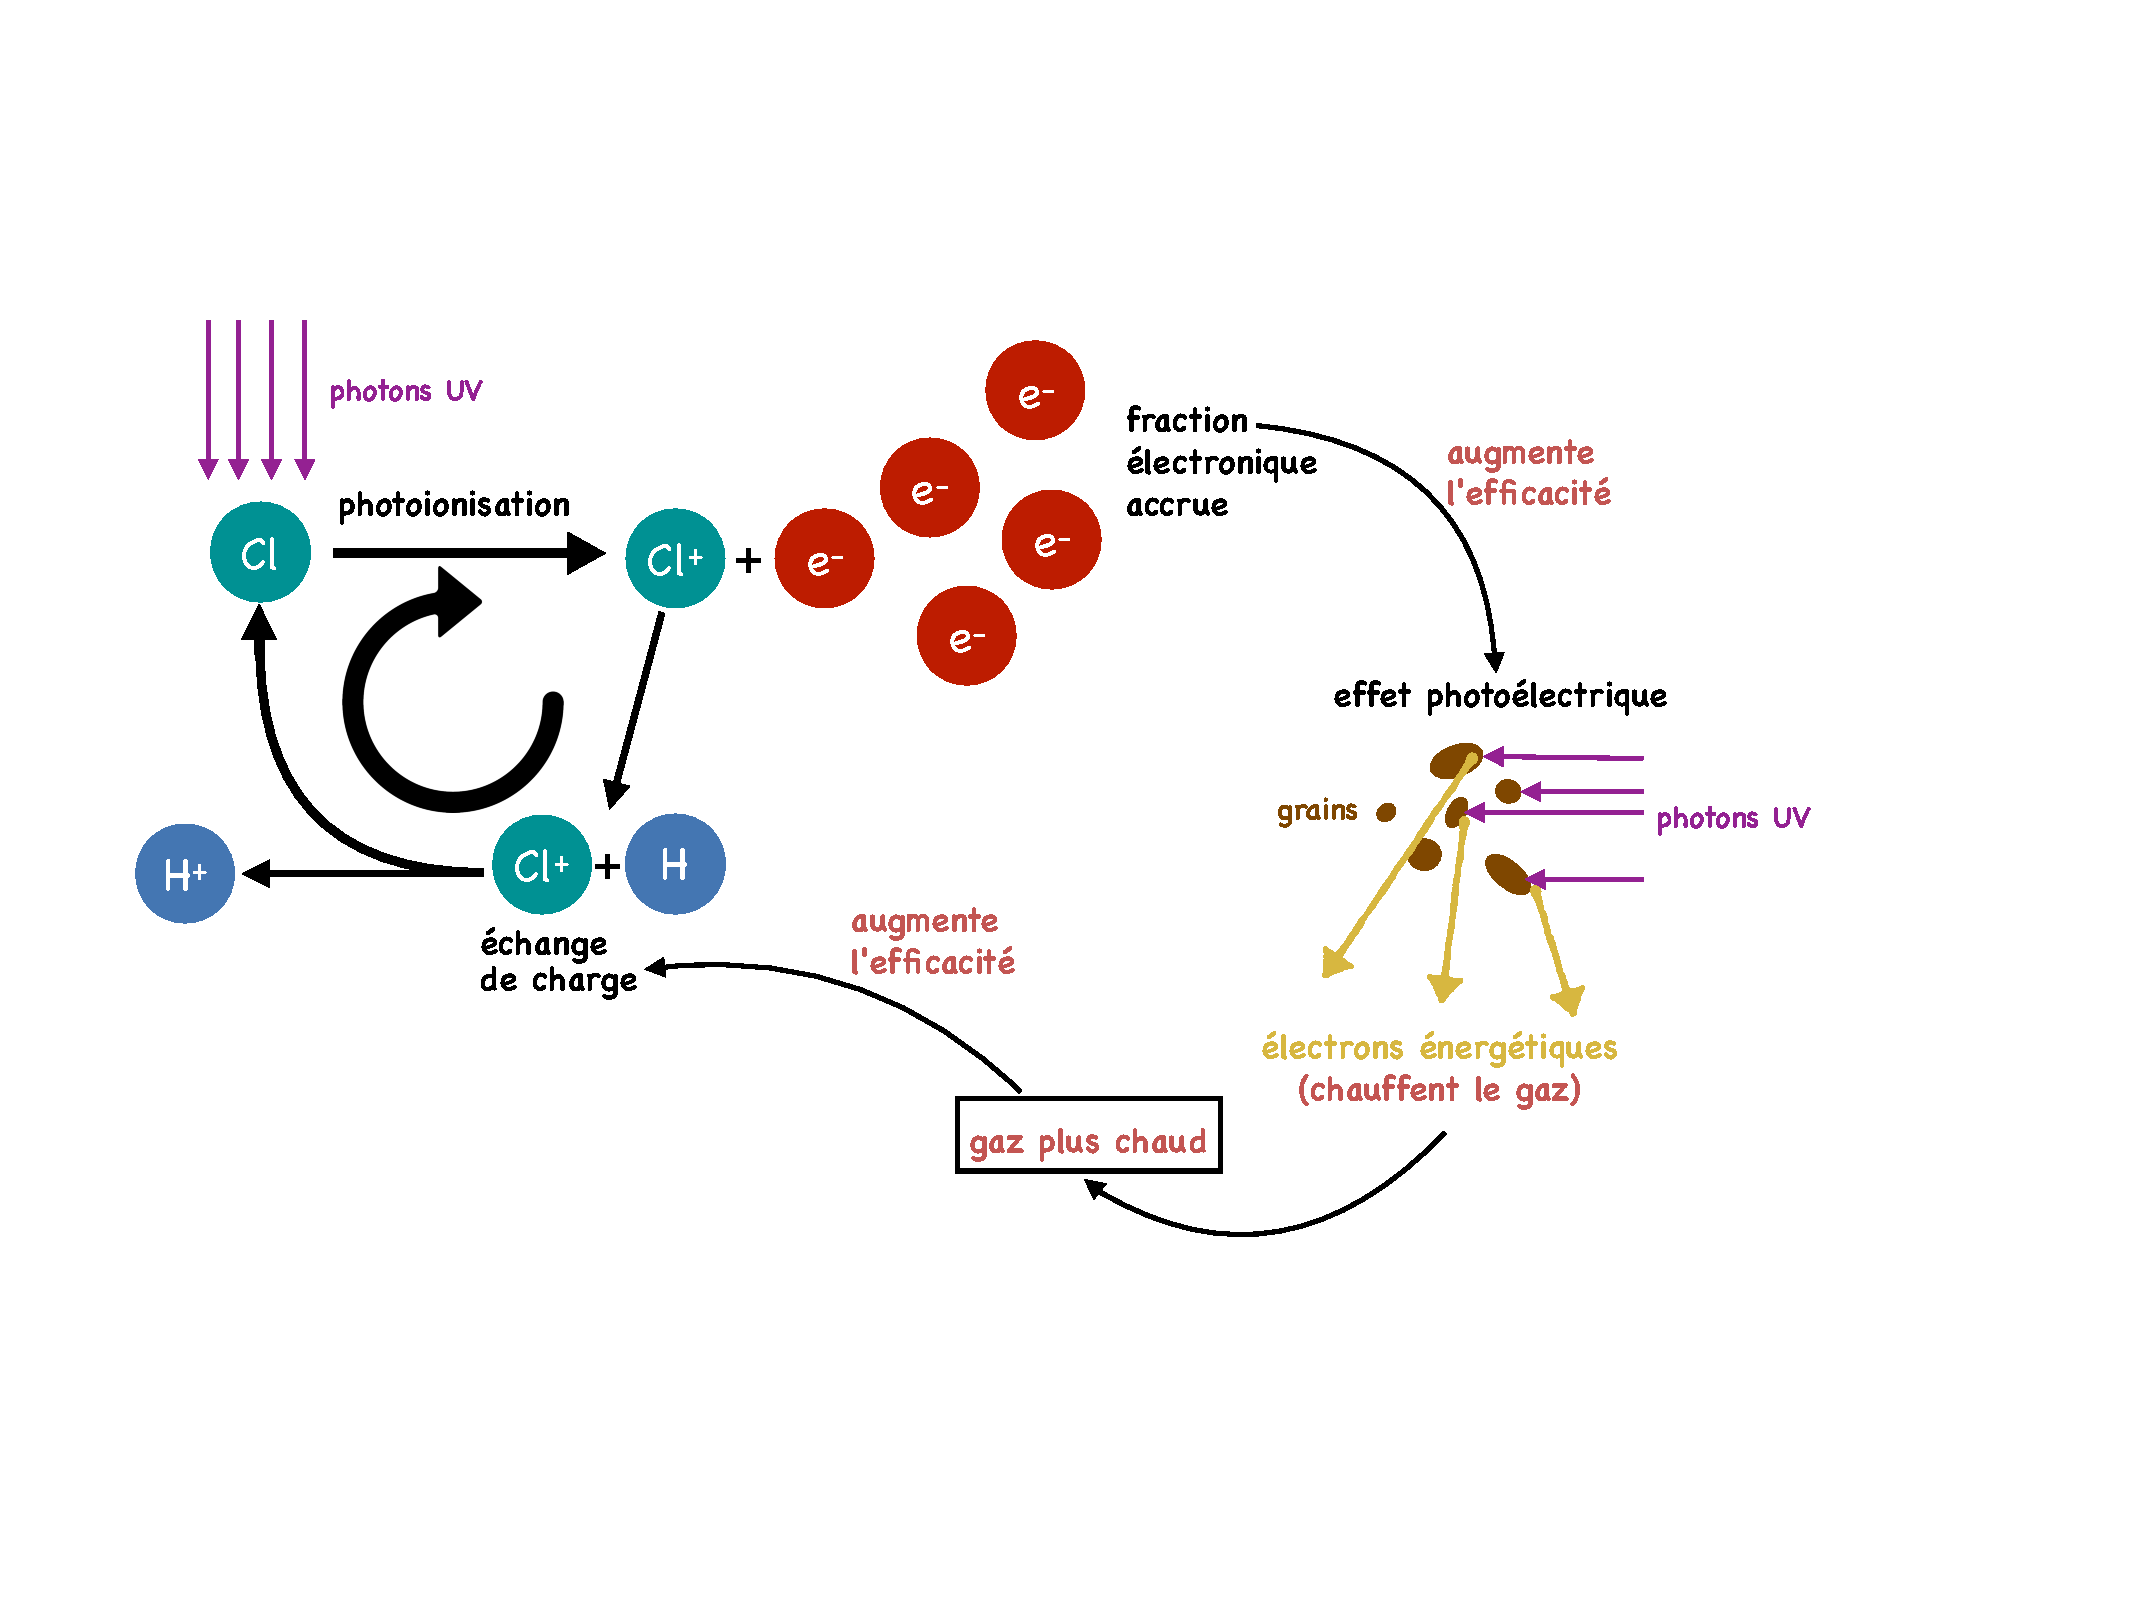
\includegraphics[trim = {2cm 5cm 4cm 4cm},clip, width=0.8\textwidth]{figure/Cl/Cl_heating_fr-5.pdf}
    \caption{Schéma représentant l'impact du chlore sur la chimie de bord de nuage atomique}
    \label{fig:catalyseur}
\end{figure}{}

L'emballement de l'effet photoélectrique se produit à partir de 1000 K. Or la photoionisation du carbone et du soufre produit les électrons en bord de nuage atomique indépendamment de la température. Il existe une température où le transfert de charge devient suffisamment efficace pour que la fraction d'électrons créée via le chlore devienne dominante devant celle de la ionisation du carbone et du soufre et amorce la rétroaction de l'effet photoélectrique. L'amplification dépend donc l'énergie d'activation du transfert de charge $\mathrm{Cl}^+  + \mathrm{H}    \rightarrow \mathrm{Cl}   +  \mathrm{H}^+$ qui vaut 6290 K. \newline

Parmi les espèces figurant dans le modèle, la carbone, le soufre, le silicium ou le fer ont également un potentiel de ionisation inférieur à celui de l'hydrogène (\autoref{tab:gaz}). Pourtant aucun ne peut effectuer un transfert de charge avec l'hydrogène qui est l'espèce majoritaire en bord de nuage atomique. Ces espèces ne peuvent pas donc pas provoquer un emballement similaire à celui induit par le chlore. 



%%%%%%%%%%%%%%%%%%%%%%%%%%%%%%%%%%%%%%%%%%%%%%%%%%%%%%%%%%%%%%%%%%%%%%%%%%%%%%%%%%%%%%%%%%%%%%%

\subsection{Modèle analytique - Chimie}

Les espèces qui contribuent à la production d'électrons en bord de nuage sont les ions hydrogènes $\mathrm{H}^+$, carbones $\mathrm{C}^+$ et soufres $\mathrm{S}^+$. On peut supposer qu'en entrée de nuage atomique le carbone et le soufre sont ionisés ce qui fournit une fraction d'électrons minimale de $10^{-4}$. Le modèle doit retrouver l'augmentation de la densité d'électrons (jusqu'à $2\ 10^{-3}$) pour des températures supérieures à 1000 K.
 
\subsubsection{Ion hydrogène}

J'ai isolé les réactions principales qui font intervenir les ions $\mathrm{H}^+$. Les réactions avec l'oxygène sont négligées car la formation et destruction de $\mathrm{H}^+$ par l'oxygène se compensent totalement en première approximation. 

\begin{equation}
    \begin{array}{lccccclr}
        \mathrm{Cl}^+ & + &\mathrm{H}   & \rightarrow &\mathrm{Cl}  & + & \mathrm{H}^+ & (k_3) \\
        \mathrm{Cl}  & + & \mathrm{H}^+  & \rightarrow & \mathrm{Cl}^+ & + &\mathrm{H}  & (k_4) \\
        \mathrm{H}^+  & + & \mathrm{e}^-  & \rightarrow &\mathrm{H}   &   &     & (k_5) \\
    \end{array}
\end{equation}

A l'état stationnaire, le bilan de formation des ions $\mathrm{H}^+$ donne
\begin{equation}\label{eq:h+}
    \frac{d}{dt}n(\mathrm{H}^+) = k_3n(\mathrm{Cl}^+)n(\mathrm{H}) - k_4n(\mathrm{Cl})n(\mathrm{H}^+) - k_5 n(\mathrm{H}^+)n(\mathrm{e}^-) = 0
\end{equation}

En introduisant la fraction atomique de chlore $\delta_{Cl}$, fixée dans le gaz, et le bilan de charge on obtient une équation en $n(\mathrm{H}^+)$ :

\begin{equation}
    -k_3n(\mathrm{Cl}^+)n_{\mathrm{H}} + \bigg( \frac{k_3 k_4}{k_1} n_{\mathrm{H}} n(\mathrm{Cl}^+) + k_5 \big(n(\mathrm{C}^+)+ n(\mathrm{S}^+)\big) \bigg) n(\mathrm{H}^+) + k_5 n(\mathrm{H}^+)^2 = 0
\end{equation}

 avec,
\begin{equation}
    \delta_{Cl} = \SI{1.8}{10^{-7}} = \frac{n(\mathrm{Cl}) + n(\mathrm{Cl}^+) + ...}{n(\mathrm{H}) + n(\mathrm{H}^+) + 2n(\mathrm{H}_2) + ...} \approx \frac{1}{n_{\mathrm{H}}} (n(\mathrm{Cl}) + n(\mathrm{Cl}^+) )
\end{equation}

On obtient une solution qui dépend de $n(\mathrm{Cl}^+)$,
\begin{equation}
\resizebox{1.1\hsize}{!}{
    \boxed{n(\mathrm{H}^+) = -\frac{1}{2} \bigg( \frac{k_3 k_4}{k_1 k_5} n_{\mathrm{H}} n(\mathrm{Cl}^+) + n(\mathrm{C}^+)+ n(\mathrm{S}^+) \bigg) \pm \frac{1}{2} \sqrt{\bigg( \frac{k_3 k_4}{k_1 k_5} n_{\mathrm{H}} n(\mathrm{Cl}^+) + n(\mathrm{C}^+)+ n(\mathrm{S}^+) \bigg)^2 + 4\frac{k_3}{k_5}n_{\mathrm{H}} n(\mathrm{Cl}^+)}}
    }
\end{equation}

% \subsubsection{Rôle de l'oxygène}
% Au vu des taux de réactions impliquant le $\mathrm{H}^+$ nous pourrions choisir d'inclure la chimie de $\mathrm{H}^+$ avec l'oxygène. A hautes températures, les taux de $ \mathrm{H}^+ + O \leftrightarrows\mathrm{H}+ O^+ \quad (k_6,k_7)$ prédominent sur les autres réactions. Si l'on considère que ces réactions pour la chimie de l'oxygène, les $\mathrm{H}^+$ produits seront consommés pour former du $H$. Rien ne se passe. Pour s'en convaincre il suffit d'écrire la nouvelle équation bilan de $\mathrm{H}^+$ et d'utiliser celle pour $O^+$.

% \begin{equation}
%     \frac{d}{dt}n(O^+) = k_6 n(\mathrm{H}^+)n(O) - k_7n(\mathrm{H})n(O^+) = 0
% \end{equation}

% En l'injectant dans le nouveau bilan de formation pour le $\mathrm{H}^+$, ces nouveaux termes disparaissent. Cependant si l'on calcule l'expression de $n(\mathrm{H}^+)$ à partir des concentrations de $n(O^+)$ et $n(O)$, l'approximation donne une meilleure correspondance avec l'abondance calculé par le code. 

% \begin{equation}
%     n(\mathrm{H}^+) =  \frac{k_3 n_{\mathrm{H}} n(\mathrm{Cl}^+) + k_6 n_{\mathrm{H}} n(O^+) }{k_5 n(\mathrm{e}^-) + k_4 \frac{n(\mathrm{Cl}^+)}{A} + k_7 n(O) }
% \end{equation}

% Utiliser les abondances de l'oxygène demande d'étudier sa chimie, et donc de prendre en compte d'autres espèces comme $OH$ ou $O_2$ ce qui complexifie le modèle. 

%%%%%%%%%%%%%%%%%%%%%%%%%%%%%%%%%%%%%%%%%%%%%%%%%%%%%%%%%%%%%%%%%%%%%%%%%%%%%%%%%%%%%%%%%%%%%%

\subsubsection{Ion chlore}

La recombinaison électronique de $\mathrm{Cl}^+$ reste négligeable devant le transfert de charge avec $\mathrm{H}$ pour des températures supérieure à $100$K et la destruction par formation du $\mathrm{HCl}^+$ devient dominante dans la gamme de température $100-1000$K. Négliger ces réactions donne une approximation correcte de la densité d'ion chlore pour les régimes de températures $T\geq 1000$ K et garde l'emballement de l'effet photoélectrique. On considère ainsi les réactions ci-dessus :


\begin{equation}
    \begin{array}{lccccclr}
       \mathrm{Cl}  & + & h\nu & \rightarrow & \mathrm{Cl}^+ & + & \mathrm{e}^- & (k_1) \\
        \mathrm{Cl}^+ & + &\mathrm{H}   & \rightarrow &\mathrm{Cl}  & + & \mathrm{H}^+ & (k_3) \\
    \end{array}
\end{equation}

Un travail similaire nous donne 
\begin{equation}
    k_1(\xi_{Cl}n_{\mathrm{H}} - n(\mathrm{Cl}^+)) - k_3 n(\mathrm{Cl}^+) n_{\mathrm{H}} = 0
\end{equation}

Ce qui fait en posant $A = \frac{k_1}{k_3 n_{\mathrm{H}}}$:

\begin{equation}
\boxed{n(\mathrm{Cl}^+) = \frac{k_1 \xi_{Cl} n_{\mathrm{H}}}{k_1 + k_3 n_{\mathrm{H}}} = \frac{A}{1 + A} \xi_{cl} n_{\mathrm{H}}}
\end{equation}


%%%%%%%%%%%%%%%%%%%%%%%%%%%%%%%%%%%%%%%%%%%%%%%%%%%%%%%%%%%%%%%%%%%%%%%%%%%%%%%%%%%%%%%%%%%%%%%

\subsection{Recombinaison de $\mathrm{H}^+$ sur les grains}

La recombinaison du $\mathrm{H}^+$ sur les grains est calculé dans le code à sa manière (type 14). Le modèle chimique sans la recombinaison surestime la densité de protons aux hautes températures. \cite{Weingartner_2001} donne un taux de recombinaison $\alpha$ (équations [5][8]). 

\begin{equation}
    \alpha_{g}\left(\mathrm{X}^{i}, \psi, T\right) \approx \frac{10^{-14} C_{0} }{1+C_{1} \psi^{C_{2}}\left(1+C_{3} T^{C_{4}} \psi^{-C_{5}-C_{6} \ln T}\right)} \quad \mathrm{cm}^{3} \mathrm{s}^{-1}
\end{equation}

avec $\psi = \frac{G_0 \sqrt{T}}{n_e}$. Les coefficients $\mathrm{C}_i$ sont des paramètres donnés dans l'article. Le bilan de formation devient : 

\begin{equation}\label{eq:h+}
    \frac{d}{dt}n(\mathrm{H}^+) = k_3n(\mathrm{Cl}^+)n(\mathrm{H}) - k_4n(\mathrm{Cl})n(\mathrm{H}^+) - k_5 n(\mathrm{H}^+)n(\mathrm{e}^-) -\alpha_{g} n(\mathrm{H}^+)n_{\mathrm{H}} = 0
\end{equation}

On obtient une équation implicite en fonction de la densité d'électrons. La solution $n_e$ vérifie :
\begin{equation}
    x = n(\mathrm{H}^+)(x) + n(\mathrm{S}^+)  + n(\mathrm{C}^+)
\end{equation}

La fonction \texttt{newton} de la librairie \texttt{scipy.optimize} vient à bout de ce système. La densité d'électrons calculée montré sur la figure \ref{fig:Cl:model:rec}. On a résolu le système dans deux cas. Un cas avec les PAH (fraction massique = $4.6\,10^{-2}$) où le taux de recombinaison donné \cite{Weingartner_2001} donne une bonne estimation de la densité d'électrons. Un second cas sans PAH, où il faut réduire d'un facteur $1/6$ la recombinaison de $\mathrm{H}^+$ sur les grains. On avait toujours $r_{\mathrm{min}} = 1\,10^{-7}\,\mathrm{m}$ et $r_{\mathrm{max}} = 3\,10^{-5}\,\mathrm{m}$.

\textit{Quel réaction réduit la densité d'électrons à très hautes températures et qui nous empêche d'avoir la tangente horizontale ?}


\begin{figure}[htbp]
    \centering
    \begin{subfigure}[t]{0.45\textwidth} % "0.45" donne ici la largeur de l'image
        \centering 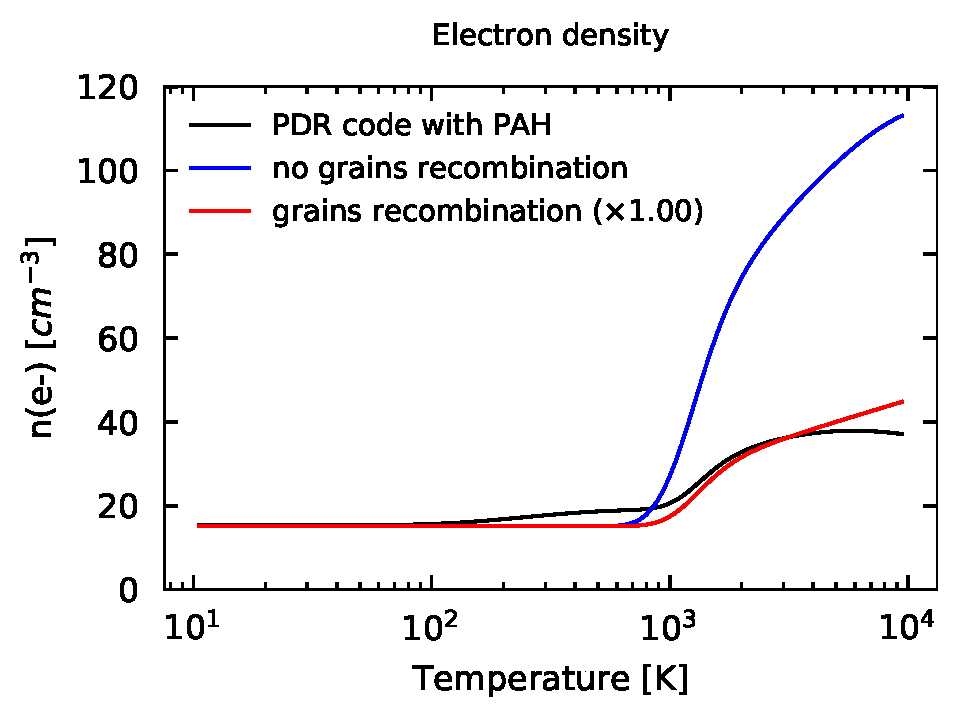
\includegraphics[trim = {0 0 0 1.5cm},clip,width=1\textwidth]{figure/Cl/model/test_calc_PAH_e.png}
        \caption{avec PAH}
    \end{subfigure}
    ~ 
    \begin{subfigure}[t]{0.45\textwidth}
        \centering 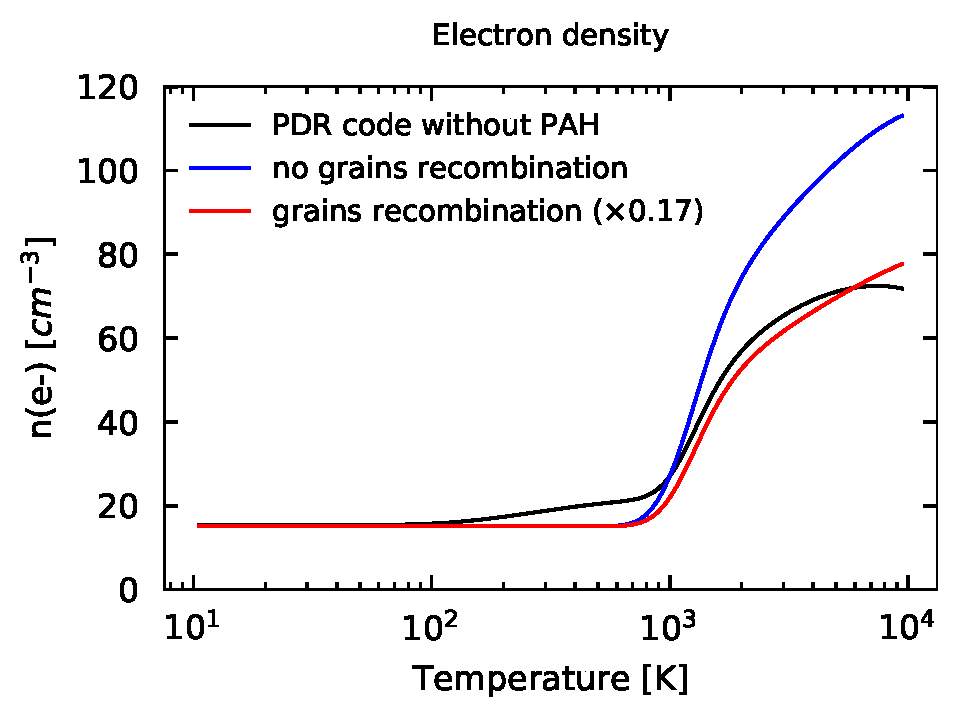
\includegraphics[trim = {0 0 0 1.5cm},clip,width=1\textwidth]{figure/Cl/model/test_calc_e.png}
        \caption{sans PAH}
    \end{subfigure}
    \caption{Profil de la densité électronique calculé par le modèle. La formule proposée par \cite{Weingartner_2001} prend en compte la recombinaison sur les PAH. Avec la recombinaison, la prédiction de la densité d'électrons est bonne dans le cas avec PAH. Si on ne prend pas en compte les PAH, il faut diminuer le taux de recombinaison d'un facteur $1/6$ pour prédire une densité d'électrons raisonnable.}
    \label{fig:Cl:model:rec}
\end{figure}



%%%%%%%%%%%%%%%%%%%%%%%%%%%%%%%%%%%%%%%%%%%%%%%%%%%%%%%%%%%%%%%%%%%%%%%%%%%%%%%%%%%%%%%%%%%%%%%
\subsection{Modèle analytique - Thermique}

On cherche la température d'équilibre du milieu dans différentes configurations de PDR. On considère dans ce modèle uniquement le chauffage par effet photoélectrique, le chauffage par $\mathrm{H}_2$ qui joue principalement dans les régions hautes densités et faible champs de rayonnement sera traité plus tard. On cherche $\Gamma = \Lambda $ en fonction de la température avec

\begin{equation}
    \begin{split}
        \Gamma &= \Gamma_{pe}^{\mathrm{Rollïg}} \\
        \Lambda &=   \Lambda_{\mathrm{CII}\ 158 \mu \mathrm{m}} + \Lambda_{\mathrm{OI}\ 63 \mu \mathrm{m}} + \Lambda_{\mathrm{OI}\ 146 \mu \mathrm{m}}  + \Lambda_{\mathrm{H}_\alpha} + \Lambda_{\mathrm{g}-\mathrm{g}} + \Lambda_{\mathrm{rec}}^{\mathrm{Rollïg}}
    \end{split}
\end{equation}


\subsubsection{Effet photoélectrique sur les grains}

De \cite{Rollig2005} (Eq (10) ou (C.3)) qui provient de \cite{BakesTielens1994}, sans PAH, on utilise : 

\begin{equation}
    \Gamma_{\mathrm{pe}} = 10^{-24}\,G_0\,n_\mathrm{H}\, \frac{2\times 10^{-2}}{1 + 2\times 10^{-4}\,G_0 \sqrt{T}/n_e} \operatorname{erg} \mathrm{cm}^{-3} \mathrm{s}^{-1}
\end{equation}

Avec $G_0 = 1.71\chi \times 0.5$ car il considère une illumination provenant que d'un coté. (\cite{Wolfire_2003} Eq 20, \cite{BakesTielens1994}) propose une autre formule prenant en compte les PAH qui est de la forme 

\begin{equation}
    \Gamma_{\mathrm{pe}}^{\mathrm{Wolf}} = 10^{-24}\,G_0\,n_\mathrm{H}\, \bbig[ \frac{4.9\times 10^{-2}}{1 + 4\times 10^{-3}\, \frac{G_0 \sqrt{T}}{n_e \phi_\mathrm{PAH}}} + \frac{3.7\times 10^{-2} (T/10^4)^{0.7}}{1 + 2\times 10^{-4}\, \frac{G_0 \sqrt{T}}{n_e \phi_\mathrm{PAH}}} \bbig] \operatorname{erg} \mathrm{cm}^{-3} \mathrm{s}^{-1}
\end{equation}

avec $\phi_\mathrm{PAH}$ une efficacité de collision compris entre 0 et 1. L'effet photoélectrique est d'autant plus efficace sur les petits grains \cite{DraineBook}. Le choix de $r_\mathrm{min}$ (la taille minimale des grains dans la description MRN) est décisif. Si l'on trace ces formules sur la \autoref{fig:Cl:pePAH} pour différent $\phi_\mathrm{PAH}$ et $r_\mathrm{min}$ on voit que la formule de \cite{Rollig2005} sous-estime le taux calculé par le code PDR de Meudon. Avec $r_\mathrm{min} = 1\,10^7\,\mathrm{nm}$, la prescription de Rollig est 3 fois plus petit que le chauffage calculé par Meudon. Si l'on augmente la taille de grain minimale, on voit que cette écart diminue ce qui est normale car l'on réduit l'efficacité de l'effet photo-électrique en enlevant les petits grains. La prescription de \cite{Wolfire_2003} laisse plus de liberté à travers le $\phi_\mathrm{PAH}$ (not much to say).

\begin{figure}[!h]
    \centering
    \begin{subfigure}[t]{0.45\textwidth} % "0.45" donne ici la largeur de l'image
        \centering 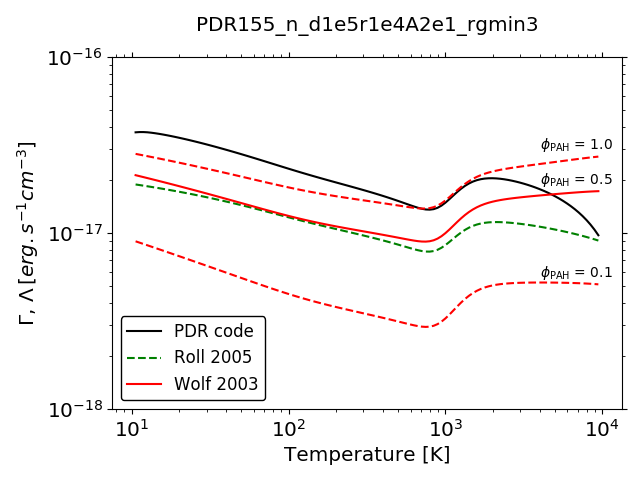
\includegraphics[trim = {0 0 0 1cm},clip,width=1\textwidth]{figure/Cl/pePAH/pe_formulae_rgmin3.png}
        \caption{$r_\mathrm{min} = 3\,10^{-7} \, \mathrm{nm}$}
    \end{subfigure}
    ~ 
   \begin{subfigure}[t]{0.45\textwidth} % "0.45" donne ici la largeur de l'image
        \centering 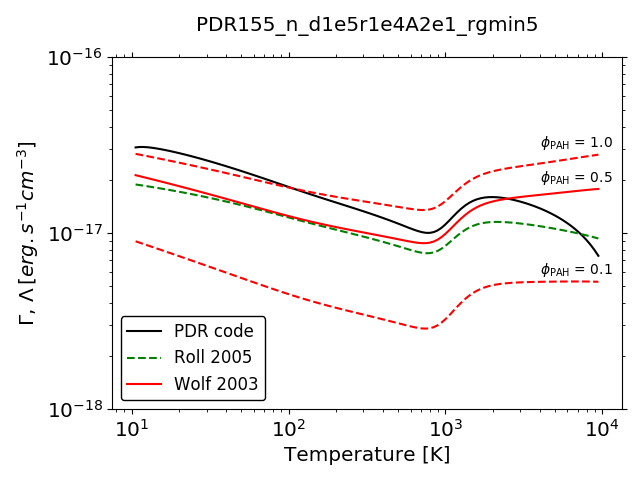
\includegraphics[trim = {0 0 0 1cm},clip,width=1\textwidth]{figure/Cl/pePAH/pe_formulae_rgmin5.png}
        \caption{$r_\mathrm{min} = 5\,10^{-7}\, \mathrm{nm}$}
    \end{subfigure}
    \caption{Comparaison des formules de l'effet photoélectrique de \cite{Rollig2005} et \cite{Wolfire_2003} avec le code PDR utilisant différents $r_\mathrm{min}$}
    \label{fig:Cl:pePAH}
\end{figure}

%%%%%%%%%%%%%%%%%%%%%%%%%%%%%%%%%%%%%%%%%%%%%%%%%%%%%%%%%%%%%%%%%%%%%%%%%%%%%%%%%%%%%%%%%%%%%%%

\subsubsection{Couplage gaz-grains}

De \cite{Rollig2005} ($Z=1$), le couplage gaz grain s'exprime,

\begin{equation}
    \Lambda_{\mathrm{g}-\mathrm{g}} = 3.5\,10^{-34}\times \sqrt{T}(T - T_g) {n_\mathrm{H}}^2 \operatorname{erg} \mathrm{cm}^{-3} \mathrm{s}^{-1}
\end{equation}

Où $T_g$ est donné par Eq. 6 de \cite{HollenbachTakahashiTielens_1991}
\begin{equation}
    T_g = 12.2 \,{G_0}^{0.2}
\end{equation}

%%%%%%%%%%%%%%%%%%%%%%%%%%%%%%%%%%%%%%%%%%%%%%%%%%%%%%%%%%%%%%%%%%%%%%%%%%%%%%%%%%%%%%%%%%%%%%%


\subsubsection{Refroidissement par les raies d'émissions du $\mathrm{C}^+$ et de $\mathrm{O}$}

[CII]$158 \mu \mathrm{m}$, provient de \cite{Rollig2005}, Equation (A.2) ($Z=1$)

\begin{equation}
    \Lambda_{\mathrm{CII}\ 158   \mu \mathrm{m}}= n(\mathrm{C}^+) \frac{2.89 \times 10^{-20}}{1+\frac{1}{2} \exp (92 / T)\left(1+\frac{1300}{n_\mathrm{H}}\right)} \operatorname{erg} \mathrm{cm}^{-3} \mathrm{s}^{-1}
\end{equation}

Pour les raies de [OI], Rollïg prend en compte les transitions adjacentes de [OI]$62 \mu \mathrm{m}$ et $[OI]146 \mu \mathrm{m}$. ($Z$,$\beta = 1$)


\begin{equation}
\begin{split}
    \Lambda_{\mathrm{OI}\ 63 \mu \mathrm{m}} &= 3.15\,10^{-14} \times 8.46\,10^{-5} \times 
    n(\mathrm{O}) \\
    & \times \frac{e^{98/T} 3 n_\mathrm{H} (n_\mathrm{H} + \beta\, n_{\mathrm{cr}_{01}} ) }{{n_\mathrm{H}}^2+ e^{98/T}(n_\mathrm{H} + \frac{1}{2} n_{\mathrm{cr}_{01}} ) (3 n_\mathrm{H} + 5\, e^{228/T} (n_\mathrm{H} + \frac{1}{2} n_{\mathrm{cr}_{12}} )) } \operatorname{erg} \mathrm{cm}^{-3} \mathrm{s}^{-1}
\end{split}
\end{equation}

\begin{equation}
\begin{split}
    \Lambda_{\mathrm{OI}\ 146 \mu \mathrm{m}} &= 1.35\,10^{-14} \times 8.46\,10^{-5} \times 
    n(\mathrm{O}) \\
    & \times \frac{ {n_\mathrm{H}}^2 }{n_\mathrm{H}^2+ e^{98/T}(n_\mathrm{H} + \frac{1}{2} n_{\mathrm{cr}_{01}} ) (3 n_\mathrm{H} + 5\, e^{228/T} (n_\mathrm{H} + \frac{1}{2} n_{\mathrm{cr}_{12}} )) } \operatorname{erg} \mathrm{cm}^{-3} \mathrm{s}^{-1}
\end{split}
\end{equation}

Avec $n_{\mathrm{cr}_{01}}(T) = \frac{1.66\,10^{-5} }{1.35\,10^{-11} T^{0.45}} $ et $n_{\mathrm{cr}_{12}}(T) = \frac{8.46\,10^{-5} }{4.37\,10^{-12} T^{0.66}} $

%%%%%%%%%%%%%%%%%%%%%%%%%%%%%%%%%%%%%%%%%%%%%%%%%%%%%%%%%%%%%%%%%%%%%%%%%%%%%%%%%%%%%%%%%%%%%%%

\subsubsection{Emission Lyman $\mathrm{H}\alpha$}

\cite{tielens2005}, Eq 2.62

\begin{equation}
    \Lambda_{\mathrm{H}\alpha} = 7.3\, 10^{-19}\,n_e\,n_\mathrm{H}\,e^{-118400/T} \operatorname{erg} \mathrm{cm}^{-3} \mathrm{s}^{-1}
\end{equation}

%%%%%%%%%%%%%%%%%%%%%%%%%%%%%%%%%%%%%%%%%%%%%%%%%%%%%%%%%%%%%%%%%%%%%%%%%%%%%%%%%%%%%%%%%%%%%%%

\subsubsection{Recombinaison des électrons sur les grains}

Dans le modèle de chlore, on prend celle de \cite{Rollig2005} Eq.4  qui provient elle même de \cite{BakesTielens1994}.

\begin{equation}
    \Lambda_{\mathrm{rec}}^{\mathrm{Rollïg}} = 3.49\,10^{-30} T^{0.944} \, (\frac{G_0 \sqrt{T}}{n_e})^{\frac{0.735}{T^{0.068}}} \, n_e \, n_\mathrm{H} \operatorname{erg} \mathrm{cm}^{-3} \mathrm{s}^{-1}
\end{equation}

Il existe également celle ci \cite{WolfireHollenbachMcKeeTielensBakes_1995} Eq. 9 que l'on n'utilise pas.

\begin{equation}
    \Lambda_{\mathrm{rec}}^{\mathrm{Wolfire}} = 4.65\,10^{-30} T^{0.94} \, (\frac{G_0 \sqrt{T}}{n_e})^{\frac{0.74}{T^{0.068}}} \, n_e \, n_\mathrm{H} \operatorname{erg} \mathrm{cm}^{-3} \mathrm{s}^{-1}
\end{equation}

%%%%%%%%%%%%%%%%%%%%%%%%%%%%%%%%%%%%%%%%%%%%%%%%%%%%%%%%%%%%%%%%%%%%%%%%%%%%%%%%%%%%%%%%%%%%%%%

\subsection{Prédiction de la température au bord de nuage}
\subsubsection{Carte de température en bord atomique du nuage}

Que fait le modèle ? On trace en fonction de la température le terme de chauffage $\Gamma$ et $\Lambda$ à partir de la densité d'électrons $n_e$ que l'on obtient à partir du modèle chimique. On cherche les $T_{eq}$ tel que $\Gamma - \Lambda  = 0$ que l'on caractérise de stable si autour du point d'équilibre $\frac{d}{dT}(\Gamma - \Lambda) <0$ et d'instable sinon. On visualise sur \autoref{fig:Cl:grid:mapT} la température maximale atteignable par le bord atomique. La zone hachurée indique les solutions instables.

\textit{Conséquences dynamiques : Hydra d'Emeric}

\begin{figure}[htbp]
    \centering
    \begin{subfigure}[t]{0.45\textwidth} % "0.45" donne ici la largeur de l'image
        \centering \includegraphics[trim = {0 0 0 1.5cm},clip,width=1\textwidth]{figure/Cl/model/mapG0nHTeq_pe_OI_CII_ggr_elecrec_lyman_OI_imp.png}
        \caption{avec chlore}
    \end{subfigure}
    ~ 
    \begin{subfigure}[t]{0.45\textwidth}
        \centering \includegraphics[trim = {0 0 0 1.5cm},clip,width=1\textwidth]{figure/Cl/model/mapG0nHTeq_pe_OI_CII_ggr_elecrec_lyman_OI_noCl.png}
        \caption{sans chlore}
    \end{subfigure}
    \caption{Carte de la température en bord de nuage atomique ($A_\mathrm{V}= 10^{-6}$) prédit par le modèle.}
    \label{fig:Cl:model:mapT}
\end{figure}

Si l'on prend en compte la recombinaison sur les grains, la prédiction des la densité d'électrons devient quantitavement proche de celle que calculerait le modèle. En retracant les cartes de températures (\autoref{}) on se rend compte qu'elles ne sont pas beaucoup modifiées.

\subsubsection{Grille de modèles}

Les grilles de modèle de la version du code \uncinq donne des cartes de température plotée sur la \autoref{fig:Cl:grid:mapT}. Le même quadrant est impacté bien que la solution haute ne soit pas toujours atteinte. La région faible champs de rayonnement et haute densité est prédominée par le chauffage par la molécule $\mathrm{H}_2$ qui n'est pas pris en compte dans ce petit modèle.  

\textit{Que se passe t'il à faible densité ? Pourquoi n'a t on pas les tangentes horizontales de T ?}

\begin{figure}[!htbp]
    \centering
    \begin{subfigure}[t]{0.45\textwidth} % "0.45" donne ici la largeur de l'image
        \centering 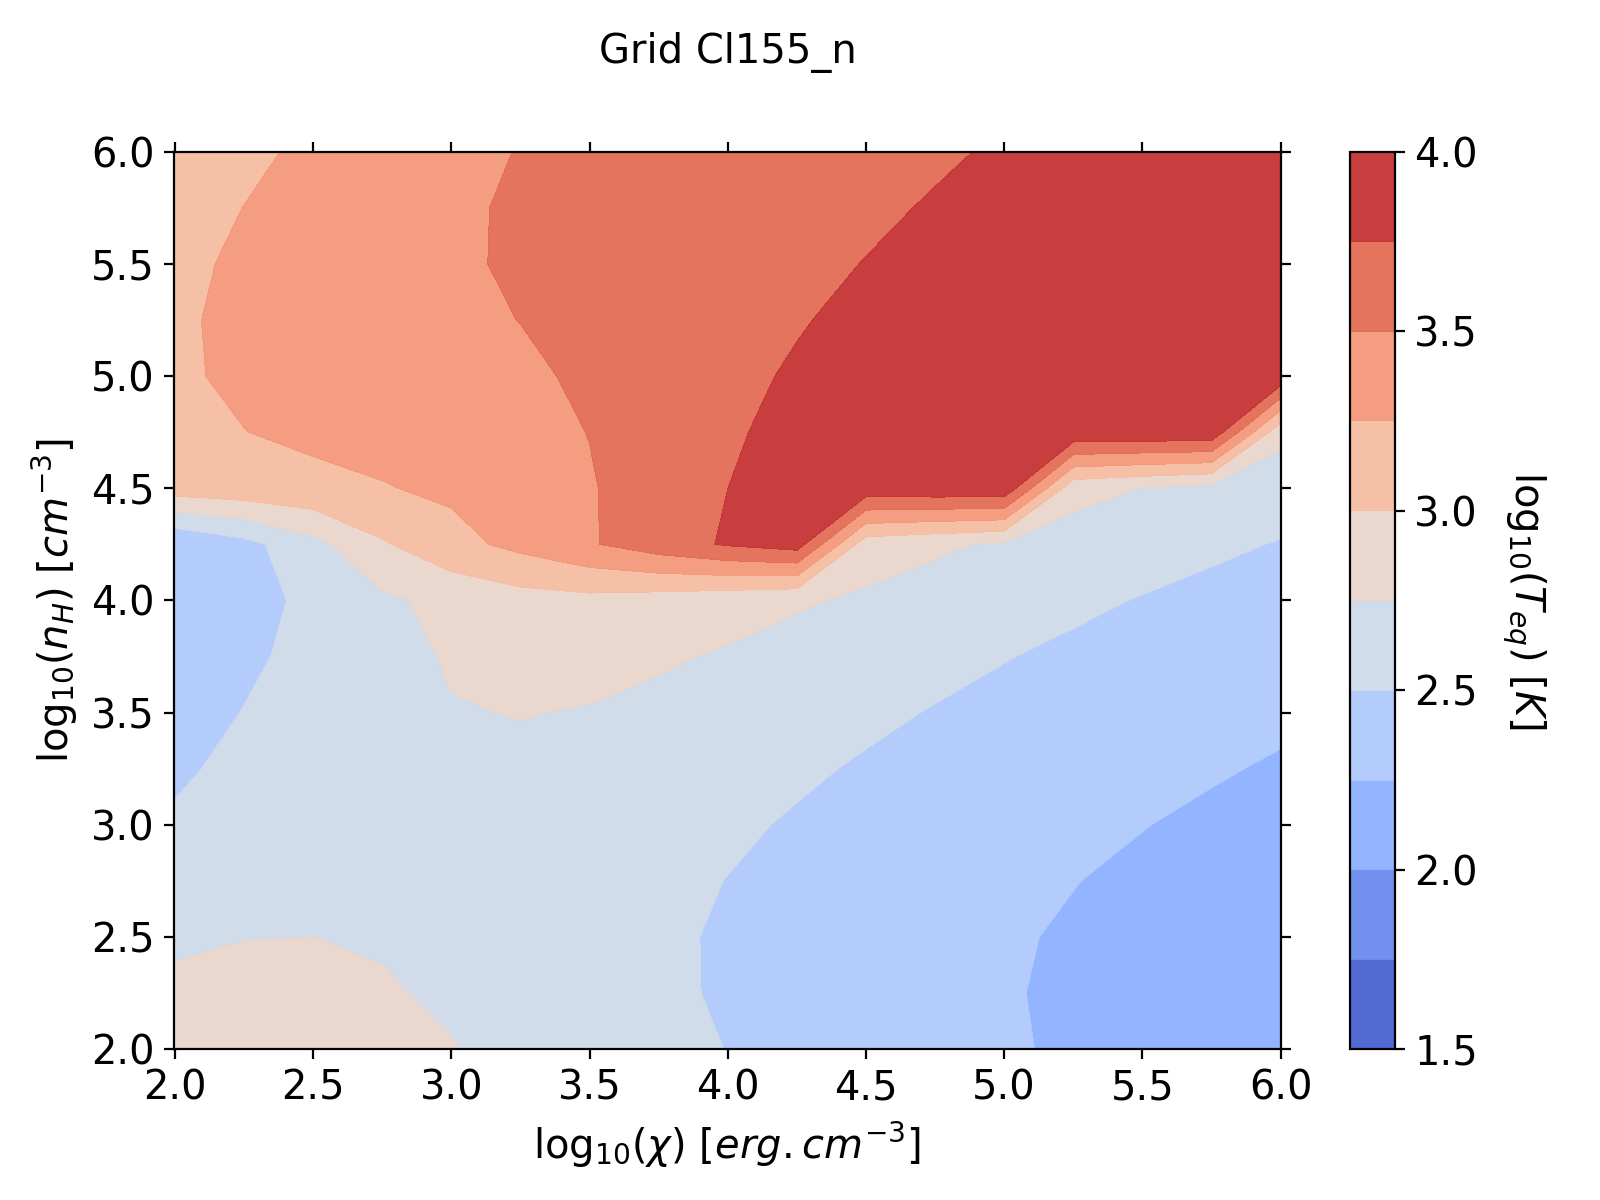
\includegraphics[trim = {0 0 0 1.5cm},clip,width=1\textwidth]{figure/Cl/grid/mapTCl.png}
        \caption{avec chlore}
    \end{subfigure}
    ~ 
    \begin{subfigure}[t]{0.45\textwidth}
        \centering 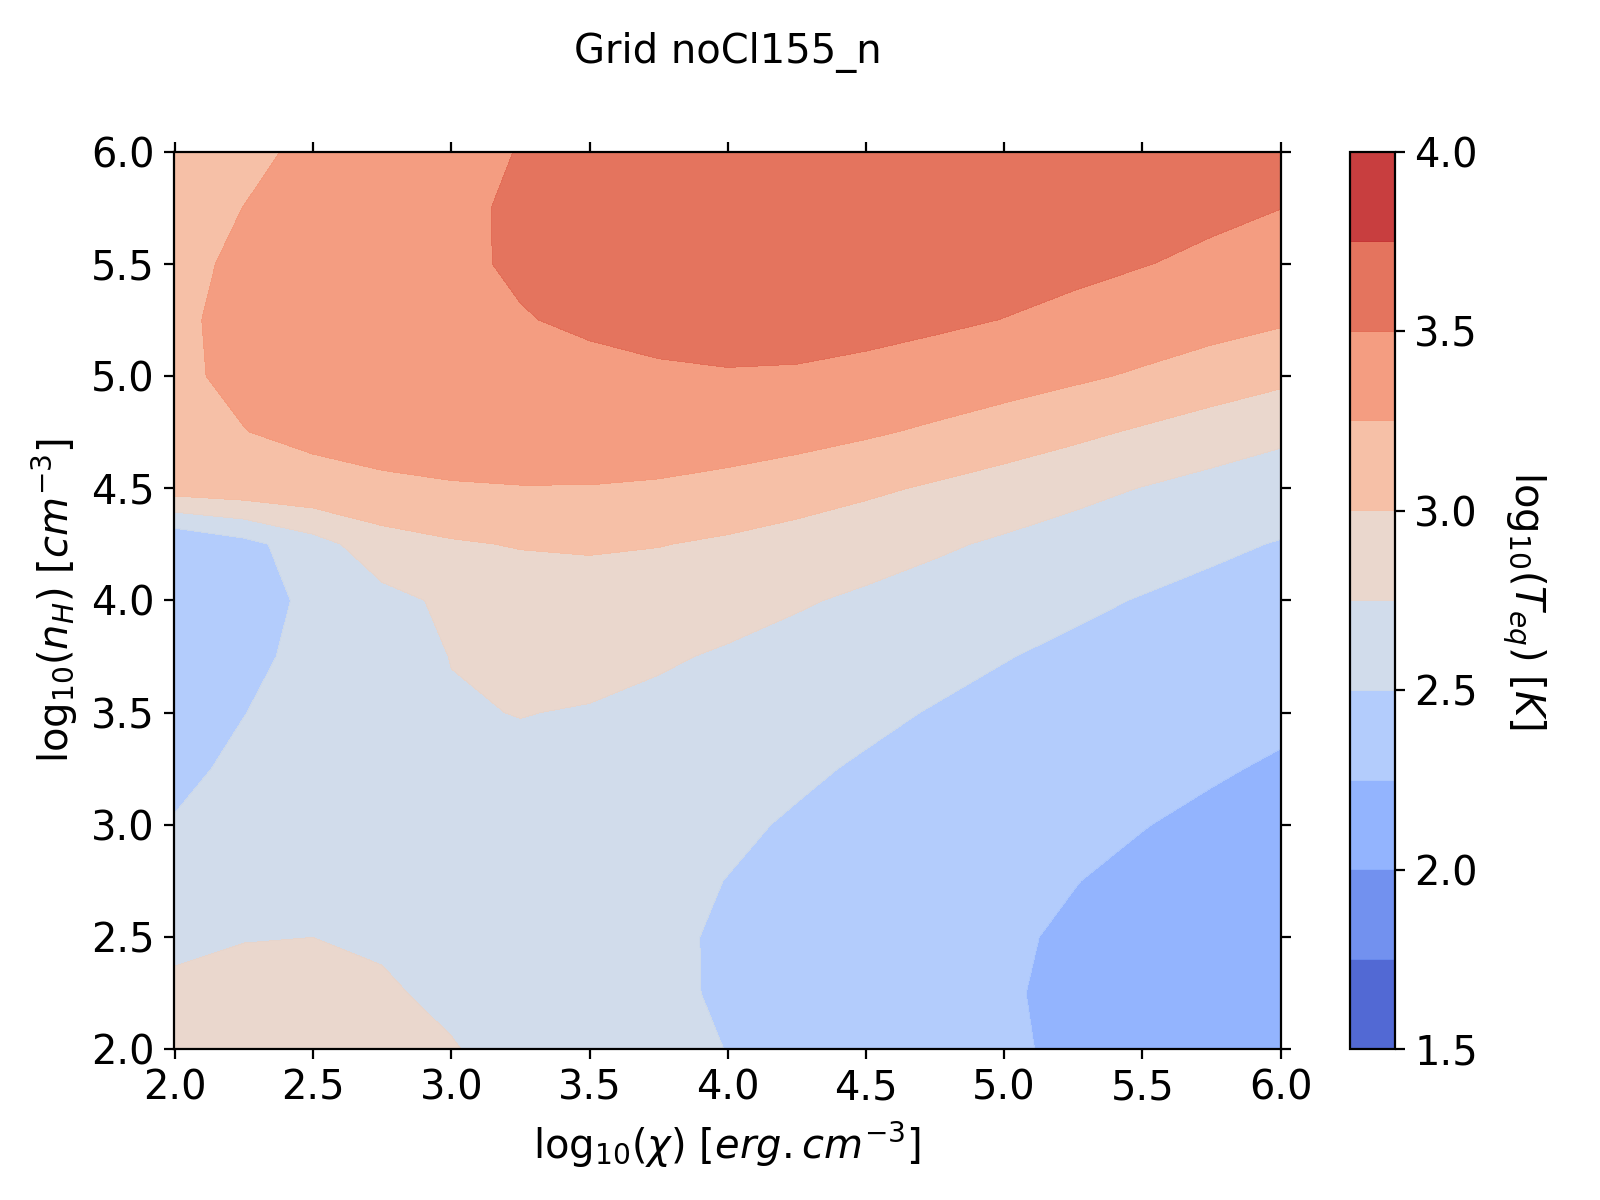
\includegraphics[trim = {0 0 0 1.5cm},clip,width=1\textwidth]{figure/Cl/grid/mapT.png}
        \caption{sans chlore}
    \end{subfigure}
    \caption{Température en bord de nuage atomique ($A_\mathrm{V}= 10^{-6}$) calculé par le code PDR \uncinq. Les PAH et la recombinaison du $\mathrm{H}^+ $ sur les grains n'ont pas été pris en compte.}
    \label{fig:Cl:grid:mapT}
\end{figure}

On a discuté précédemment de la prescription de Rollig qui sous-estime l'efficacité de l'effet photoélectrique pour des modèles de PDR avec une taille minimale de grains de $1\,10^{-7} \, \mathrm{nm}$. Si l'on corrige d'un facteur 3 le taux de chauffage c.a.d. que l'on prend un $\Gamma_{pe}^{'} = 3 \times \Gamma_{pe}^{Rollïg}$, on obtient une nouvelle carte de température assez différente.


\subsubsection{Chauffage à l'entrée du nuage moléculaire}

Il arrive qu'en entrée du nuage moléculaire, la température du gaz augmente de manière irrégulière. Dans cette région, l'effet photoélectrique devient encore plus efficace en raison de l'augmentation de la fraction électronique du nuage. La recombinaison sur les grains est rapide s'il y a une quantité importante d'électron autour des grains. Dans cette zone, le $\mathrm{H}_2$ tente de se former. La voie principale de formation passe par l'association radiative :

\begin{equation}
    \begin{array}{lccccclr}
       \mathrm{H}  & + & e^- & \rightarrow & \mathrm{H}^{-} & + & h\nu &  \\
    \end{array}
\end{equation}

suivi d'un détachement associatif :

\begin{equation}
    \begin{array}{lcccccclr}
       \mathrm{H}  & + &  \mathrm{H}^- & \rightarrow & \mathrm{H}_2 & + & e^- & + & KE\\
    \end{array}
\end{equation}

Cette réaction peut produire des électrons en quantité si elle devient dominante ce qui est le cas autour de $A_\mathrm{v} \approx 0.5 \mathrm{mag}$ sur \autoref{fig:Cl:grid:proH}. La formation du $\mathrm{H}_2$ déclenche également une chimie chaude permettant notamment de former le doux $\mathrm{CH}^+$ que l'on observe. Cette augmentation de température ne doit pas être confondue avec l'emballement provoqué par le Chlore.


\begin{figure}[!htbp]
    \centering
        \centering 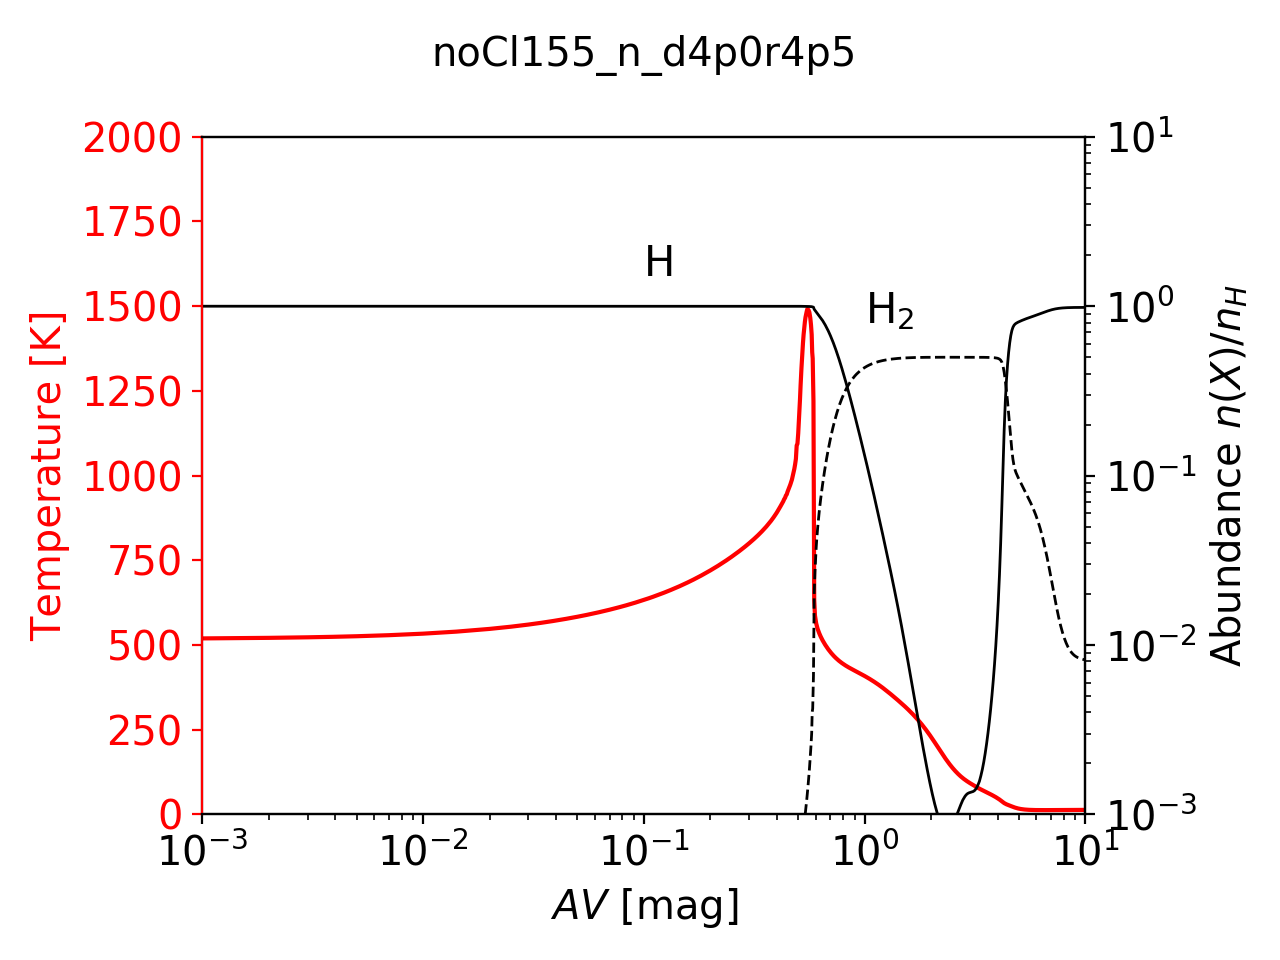
\includegraphics[trim = {0 0 0 1.5cm},clip,width=0.6\textwidth]{figure/Cl/grid/profil_H.png}
        \caption{...}
    \label{fig:Cl:grid:proH}
\end{figure}

\subsection{Diagramme d'état}

\subsection{Traceurs modifiés par le chlore}

On a pu extraire à partir des grilles calculé par le code (\uncinq) les raies d'émissions de chaques modèles et tracer des cartes d'intensités dans l'espace des paramètres et visualiser les spectres des traceurs impactés par l'ajout du chlore dans la chimie. On a étudié de 5 calculs de PDR, avec ou sans chlore, ayant des conditions physiques différentes afin de comparer localement le modèle au code de Meudon. 

\begin{figure}[!htbp]
    \centering
        \centering 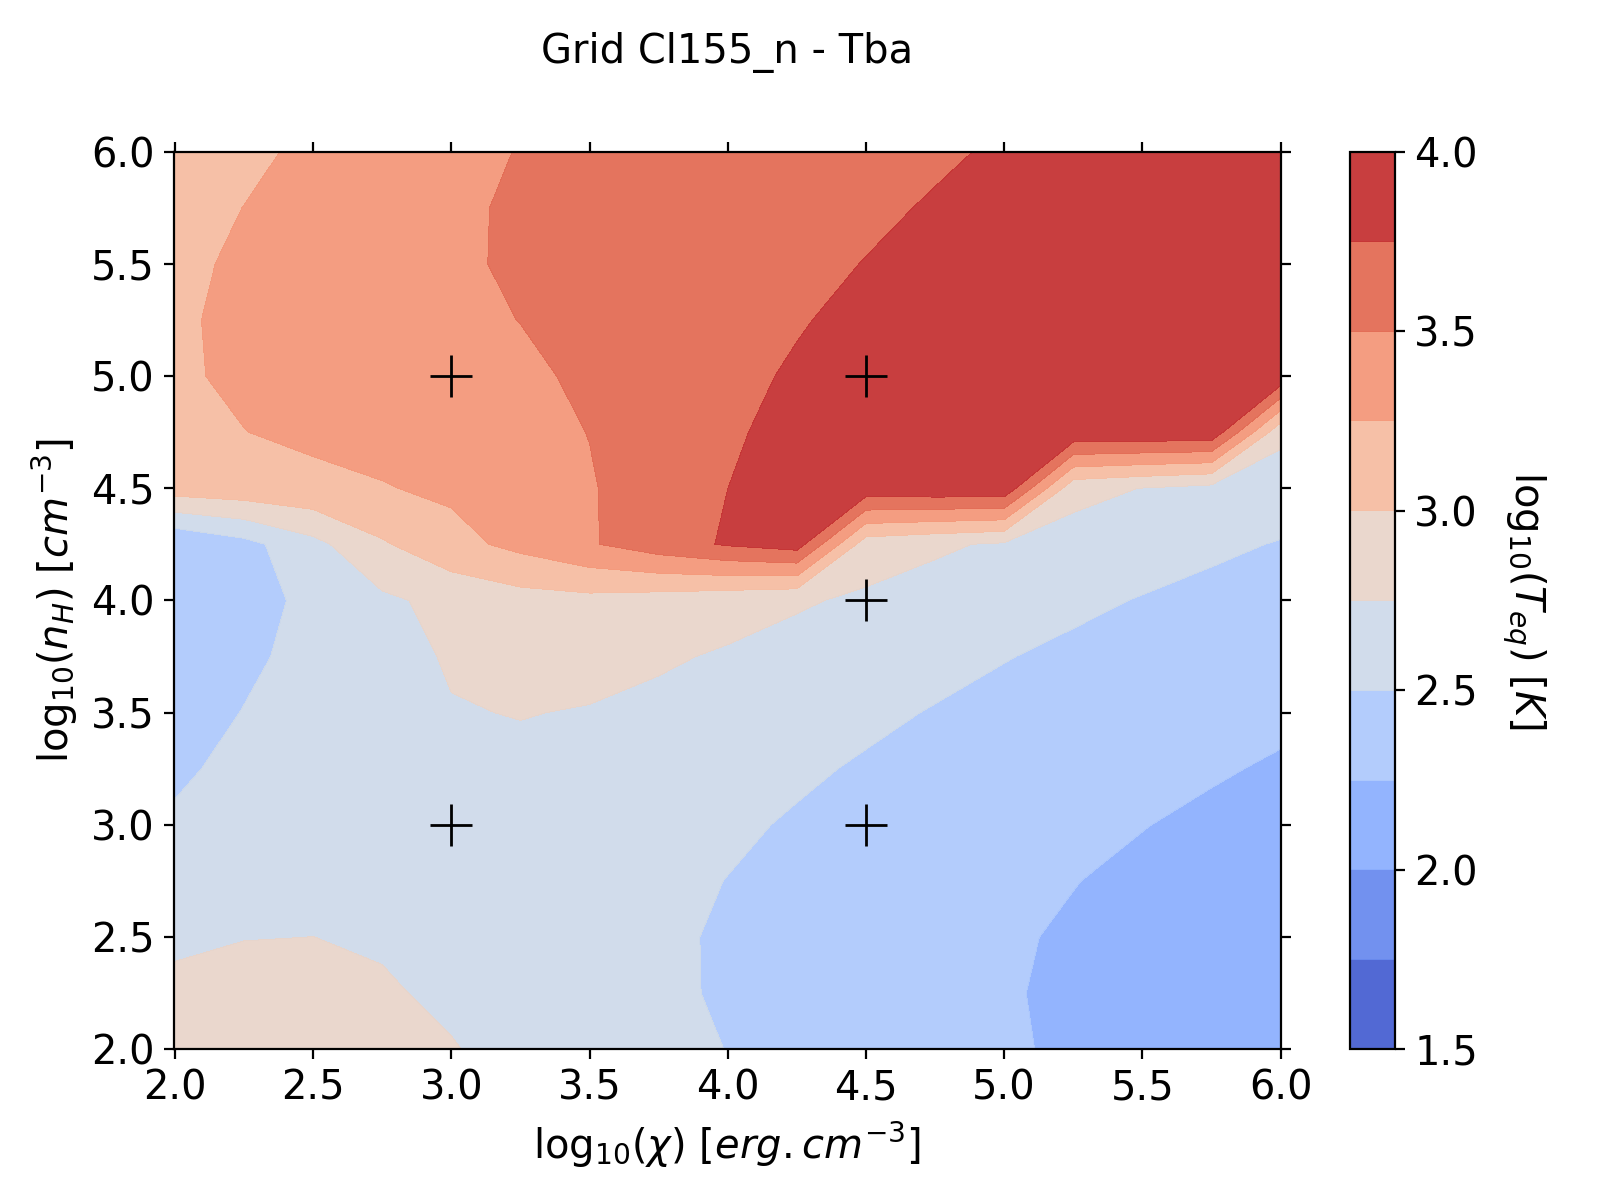
\includegraphics[trim = {0 0 0 1.5cm},clip,width=0.6\textwidth]{figure/Cl/grid/mapT_cross.png}
        \caption{...}
\end{figure}

On a compris que l'ajout du chlore : pas de signature, modifiaction des raies, facteur 3..

\subsubsection{Traceurs impactés}

Les traceurs impactés par l'ajout du chlore sont $\mathrm{N}$, $\mathrm{N}^+$, $\mathrm{S}$ et $\mathrm{Si}$. \autoref{fig:Cl:gridModelEmiss:yes}


\begin{figure}[!htbp]
    \centering
    \begin{subfigure}[t]{0.45\textwidth} % "0.45" donne ici la largeur de l'image
        \centering 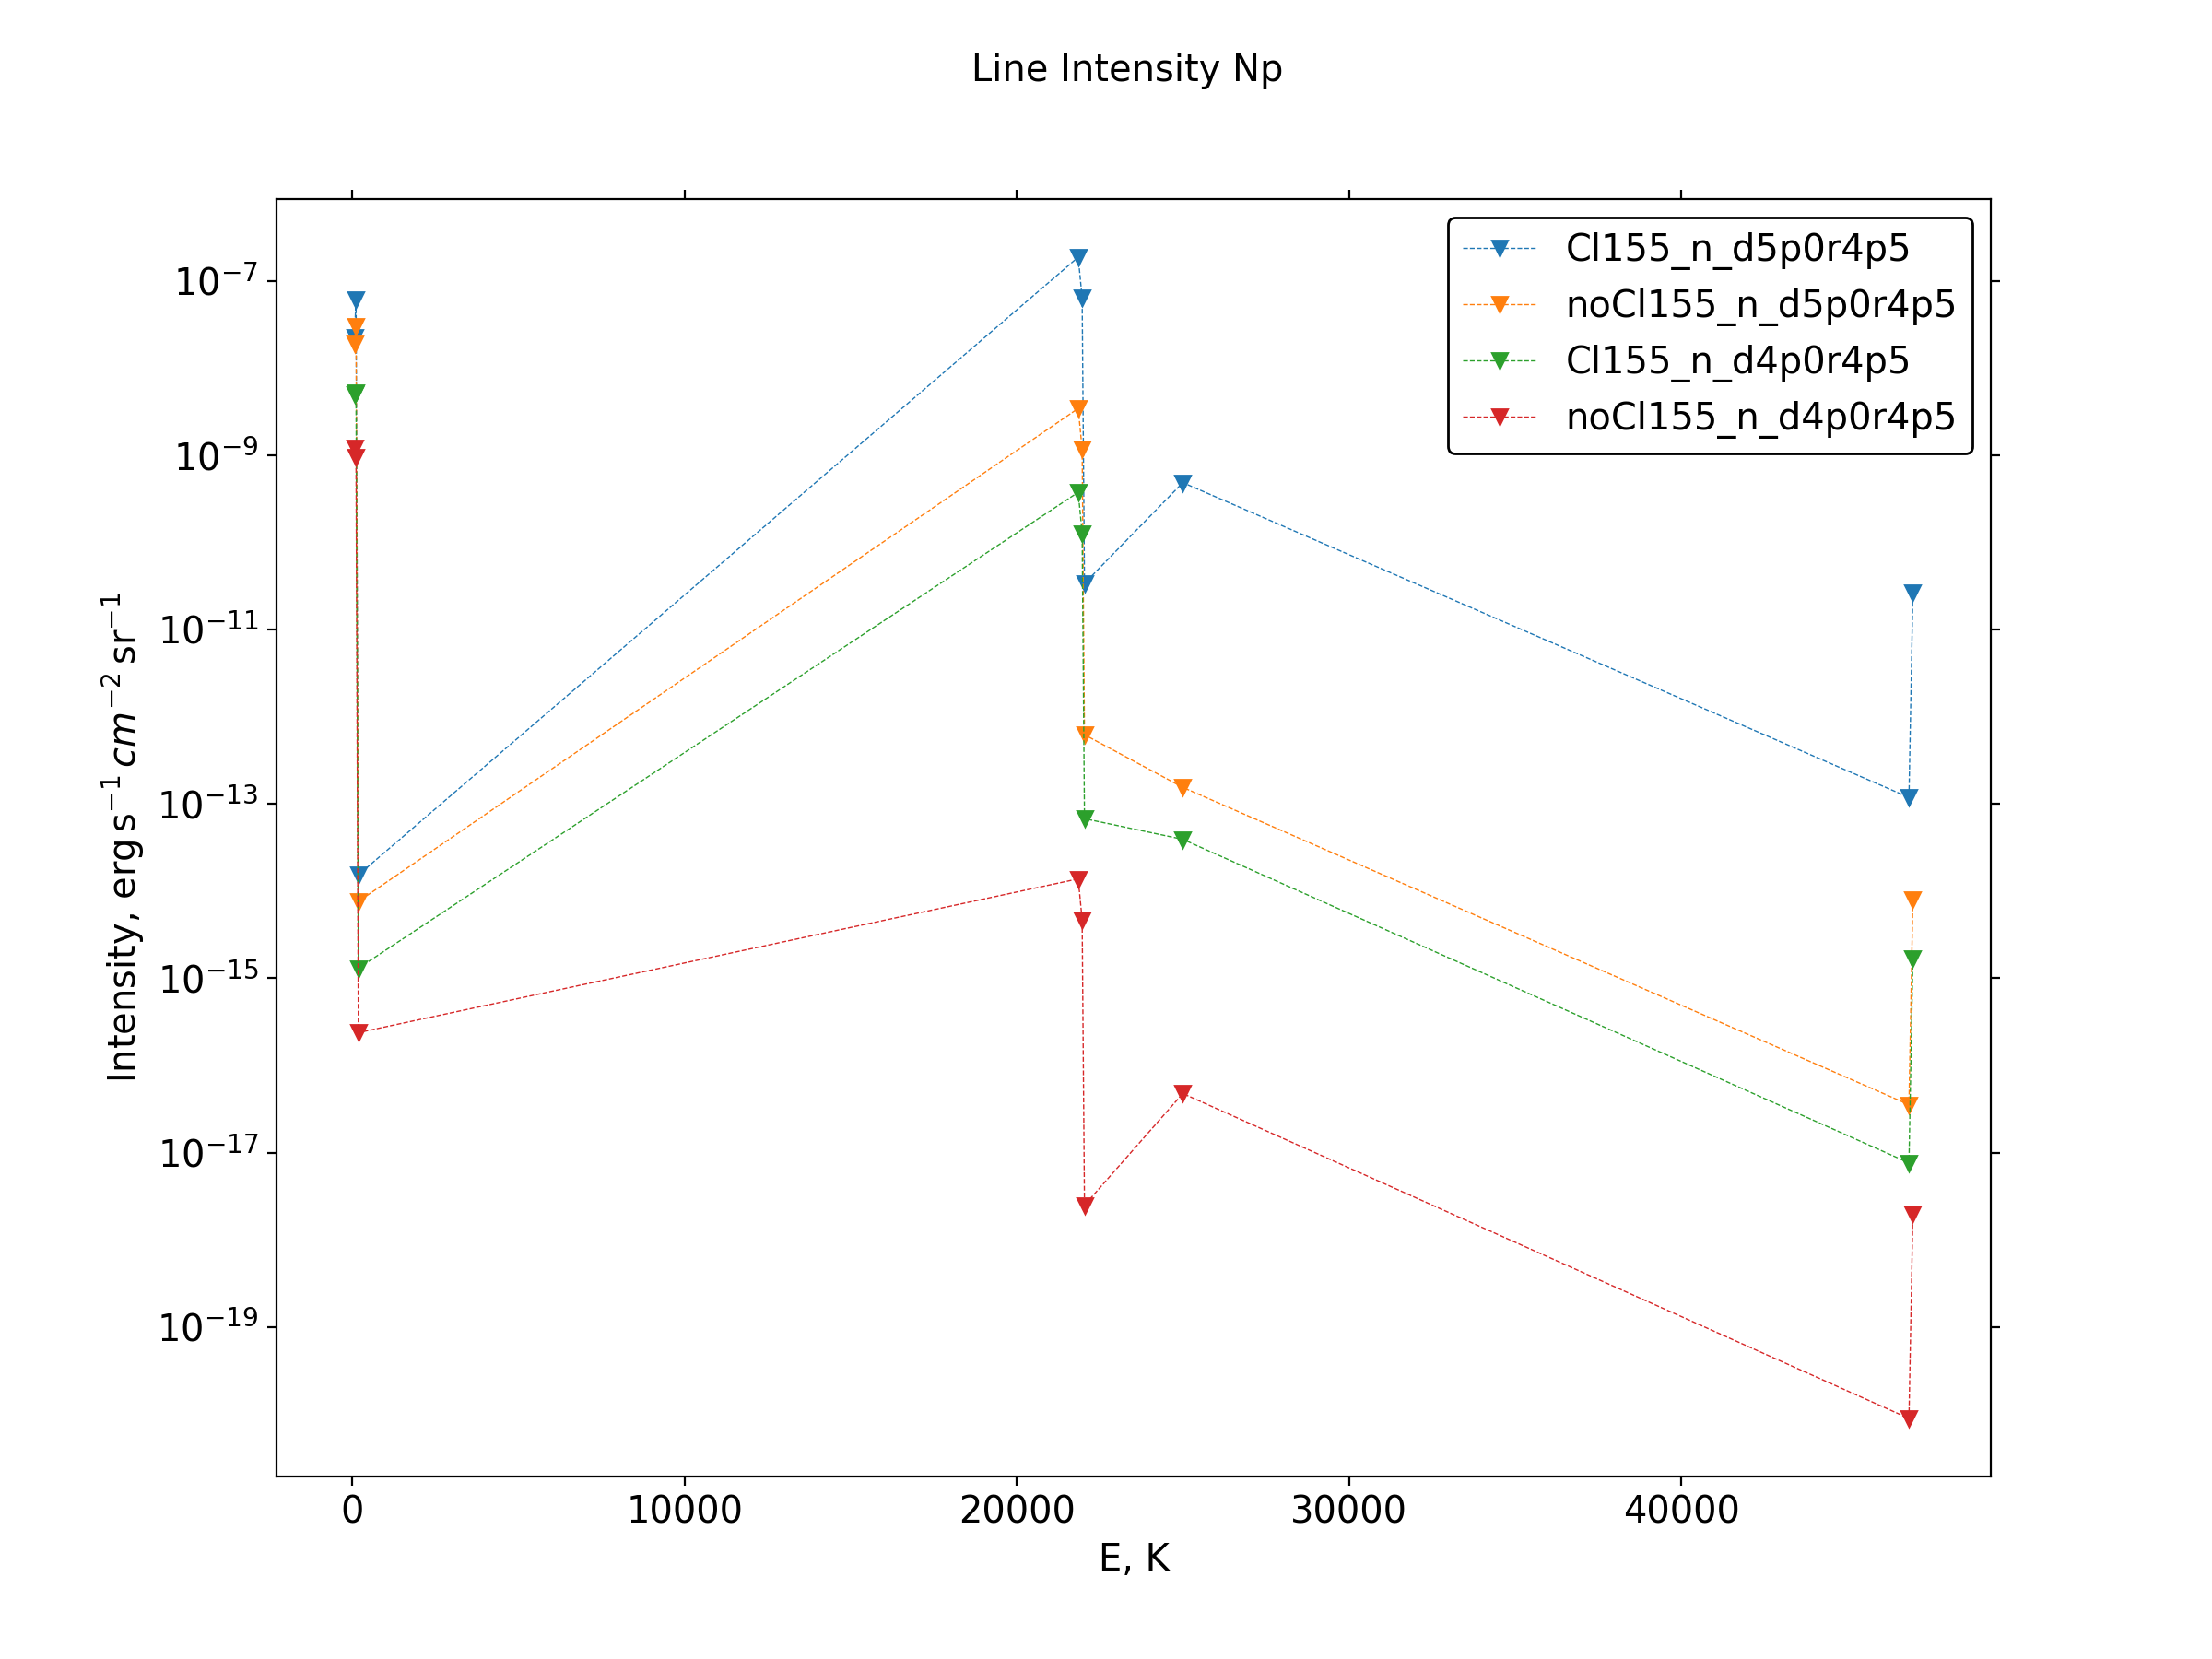
\includegraphics[trim = {0 0 0 1.5cm},clip,width=1\textwidth]{figure/Cl/gridModelEmiss/I_comp_Np.png}
        \caption{Spectre de $\mathrm{N}^+$}
    \end{subfigure}
    ~ 
   \begin{subfigure}[t]{0.45\textwidth} % "0.45" donne ici la largeur de l'image
        \centering 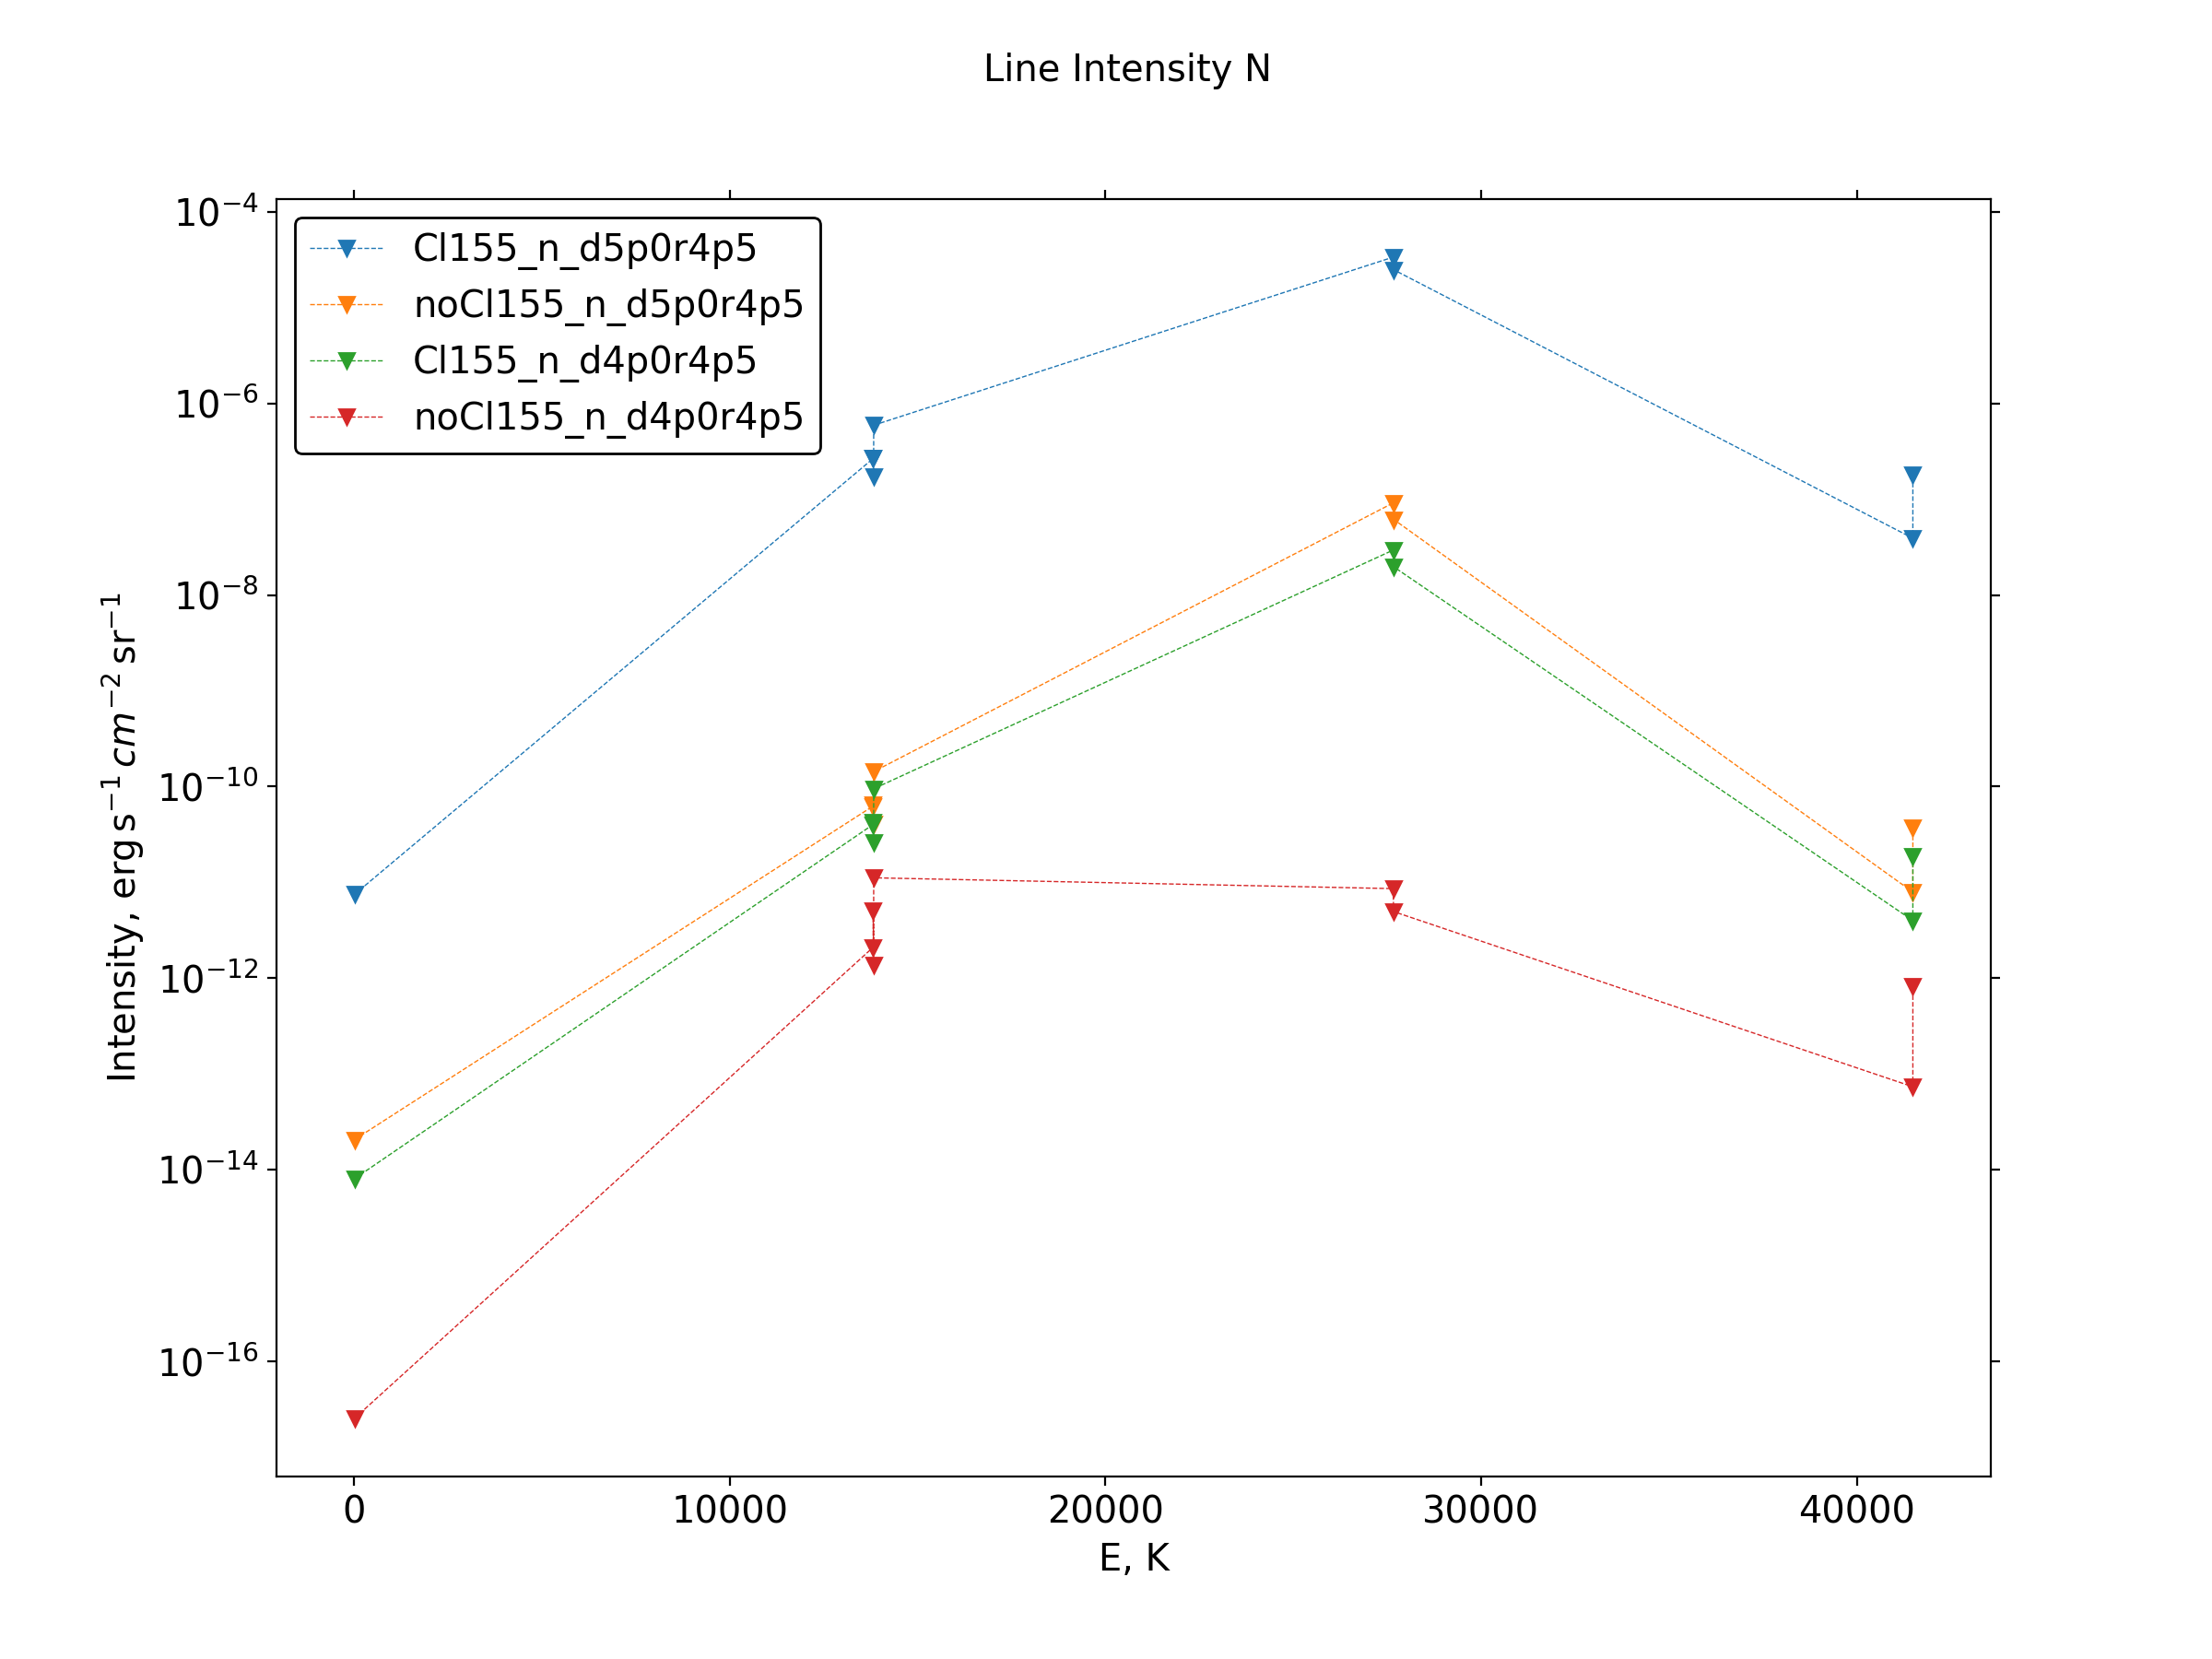
\includegraphics[trim = {0 0 0 1.5cm},clip,width=1\textwidth]{figure/Cl/gridModelEmiss/I_comp_N.png}
        \caption{Spectre de $\mathrm{N}$}
    \end{subfigure}
    
    \begin{subfigure}[t]{0.45\textwidth} % "0.45" donne ici la largeur de l'image
        \centering 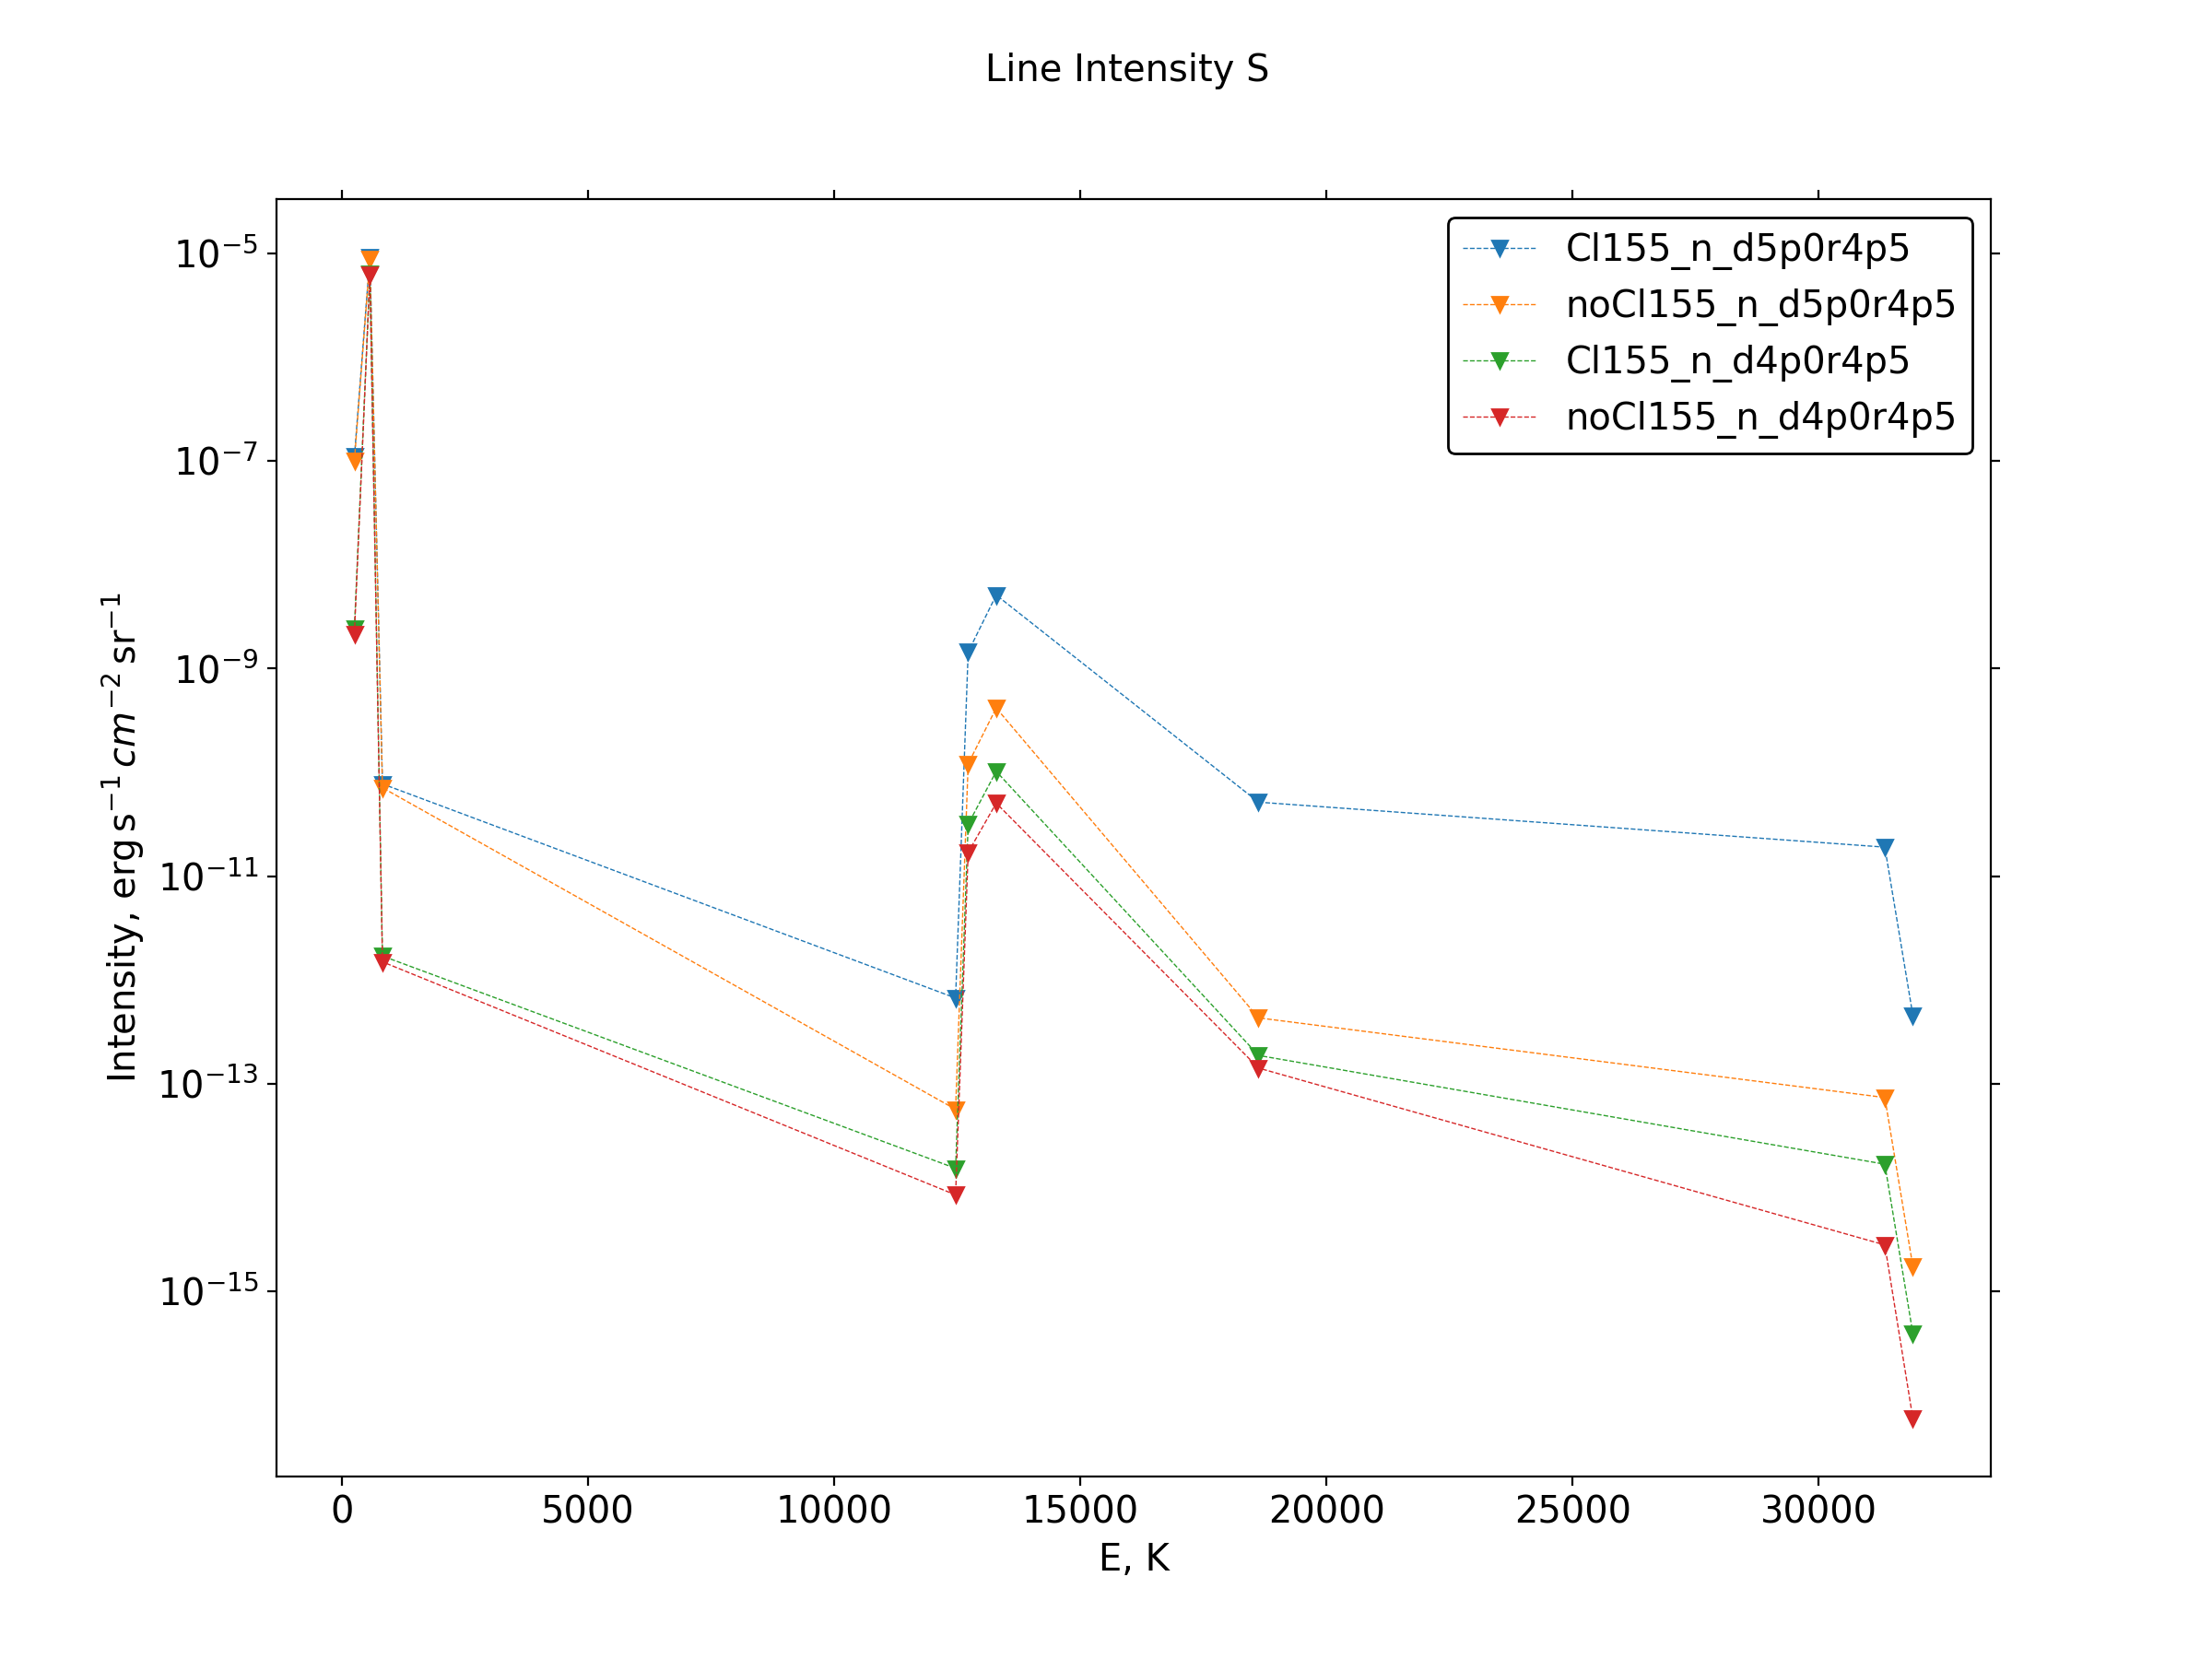
\includegraphics[trim = {0 0 0 1.5cm},clip,width=1\textwidth]{figure/Cl/gridModelEmiss/I_comp_S.png}
        \caption{Spectre de $\mathrm{S}$}
    \end{subfigure}
    ~
    \begin{subfigure}[t]{0.45\textwidth} % "0.45" donne ici la largeur de l'image
        \centering 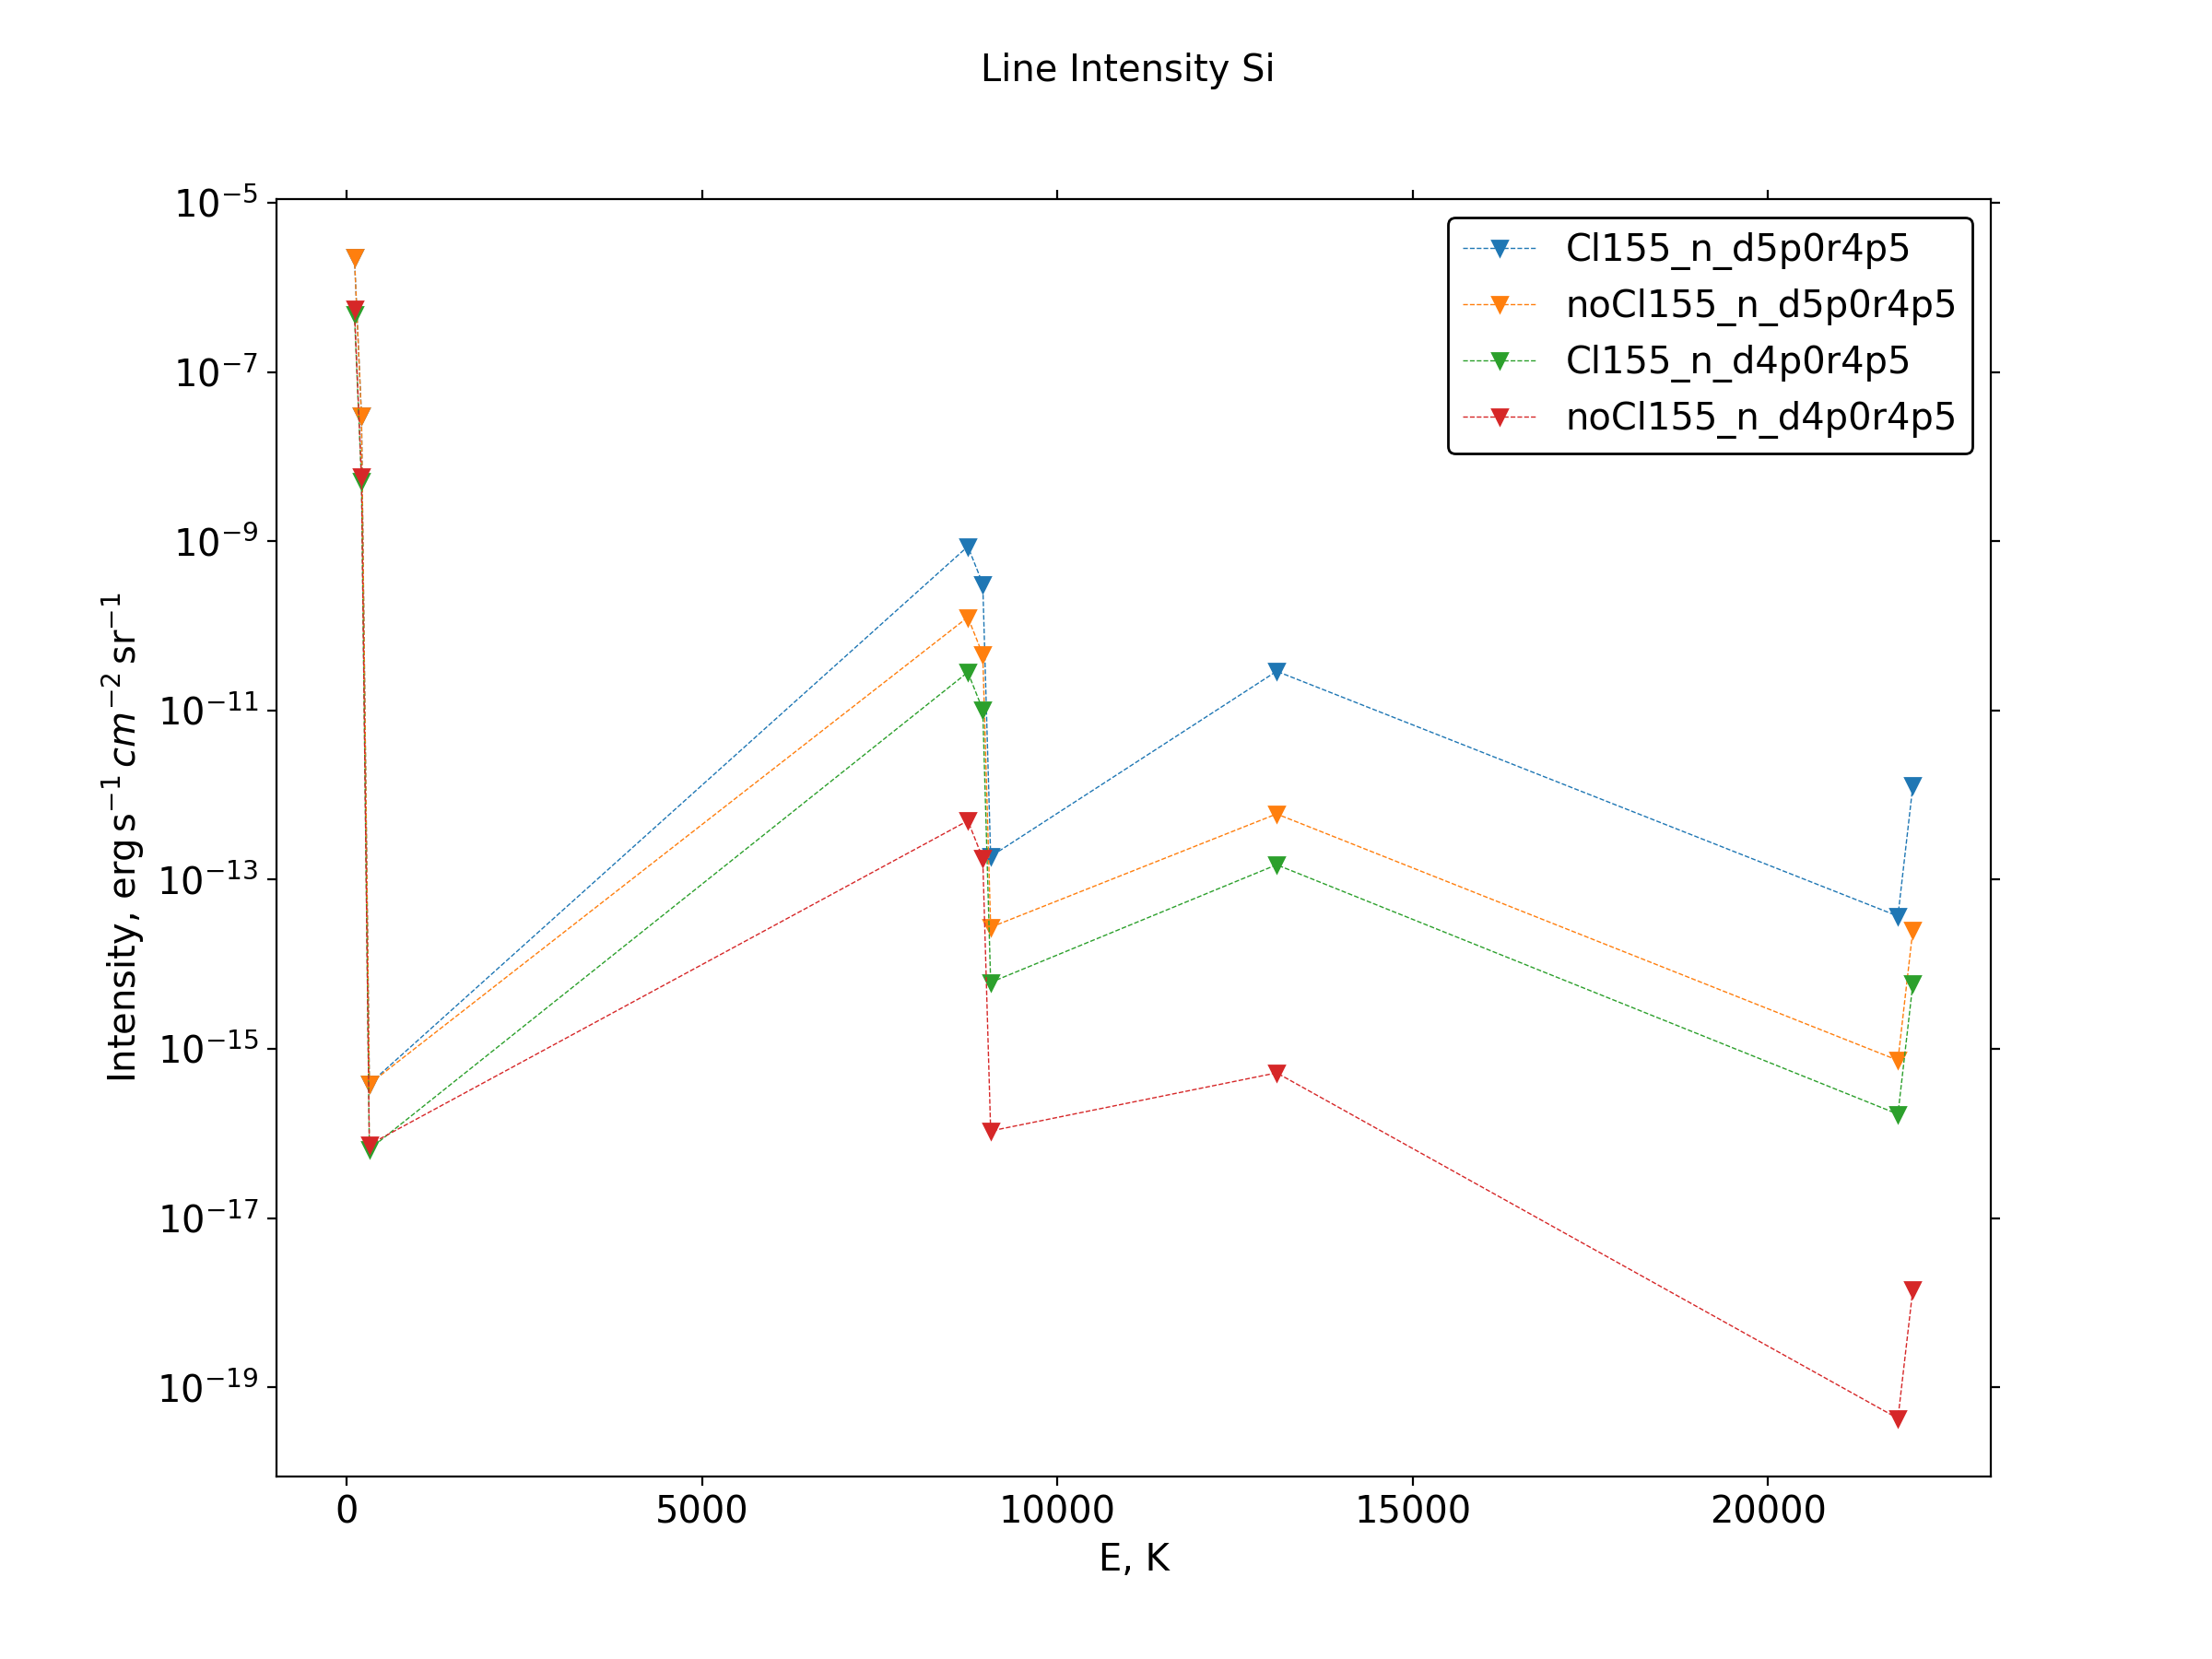
\includegraphics[trim = {0 0 0 1.5cm},clip,width=1\textwidth]{figure/Cl/gridModelEmiss/I_comp_Si.png}
        \caption{Spectre de $\mathrm{Si}$}
    \end{subfigure}
    
    \caption{Spectre chlore code PDR \uncinq}
    \label{fig:Cl:gridModelEmiss:yes}
\end{figure}



\subsubsection{$\mathrm{CS}$, $\mathrm{H}_2\mathrm{O}$}


\begin{figure}[!htbp]
    \centering
    \begin{subfigure}[t]{0.45\textwidth} % "0.45" donne ici la largeur de l'image
        \centering 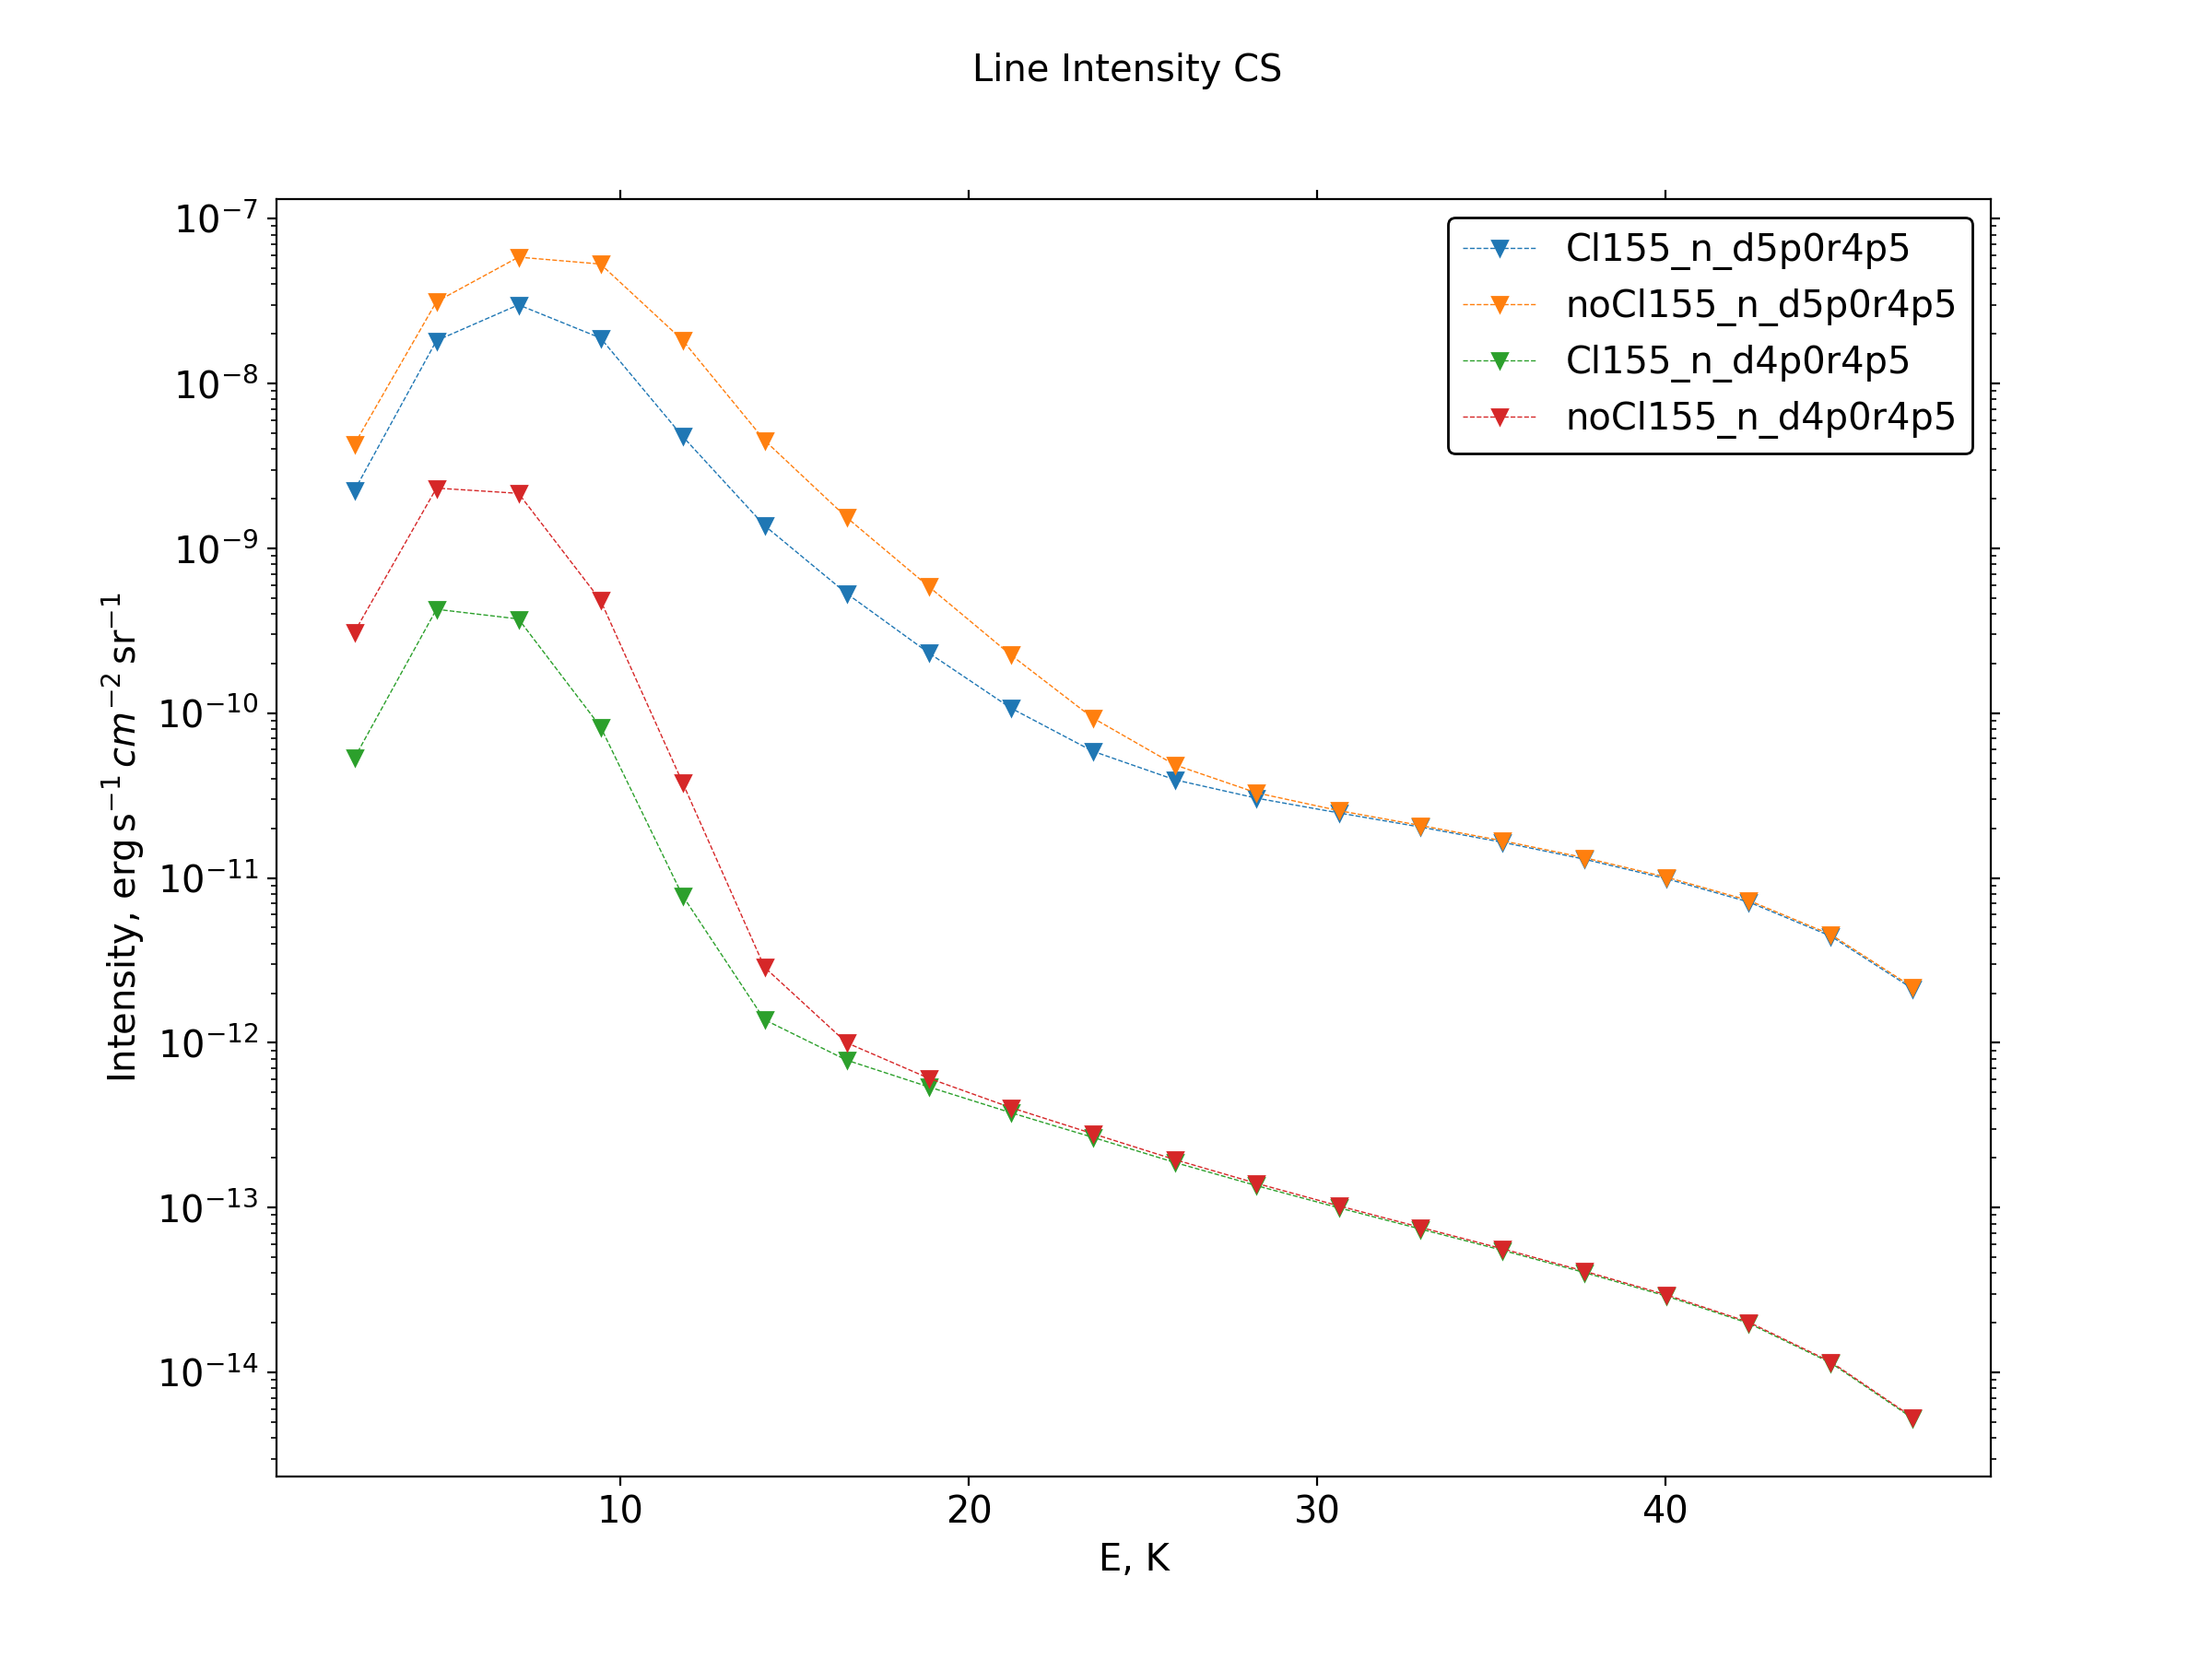
\includegraphics[trim = {0 0 0 1.5cm},clip,width=1\textwidth]{figure/Cl/gridModelEmiss/I_comp_CS.png}
        \caption{Spectre de $\mathrm{CS}$}
    \end{subfigure}
    ~ 
   \begin{subfigure}[t]{0.45\textwidth} % "0.45" donne ici la largeur de l'image
        \centering 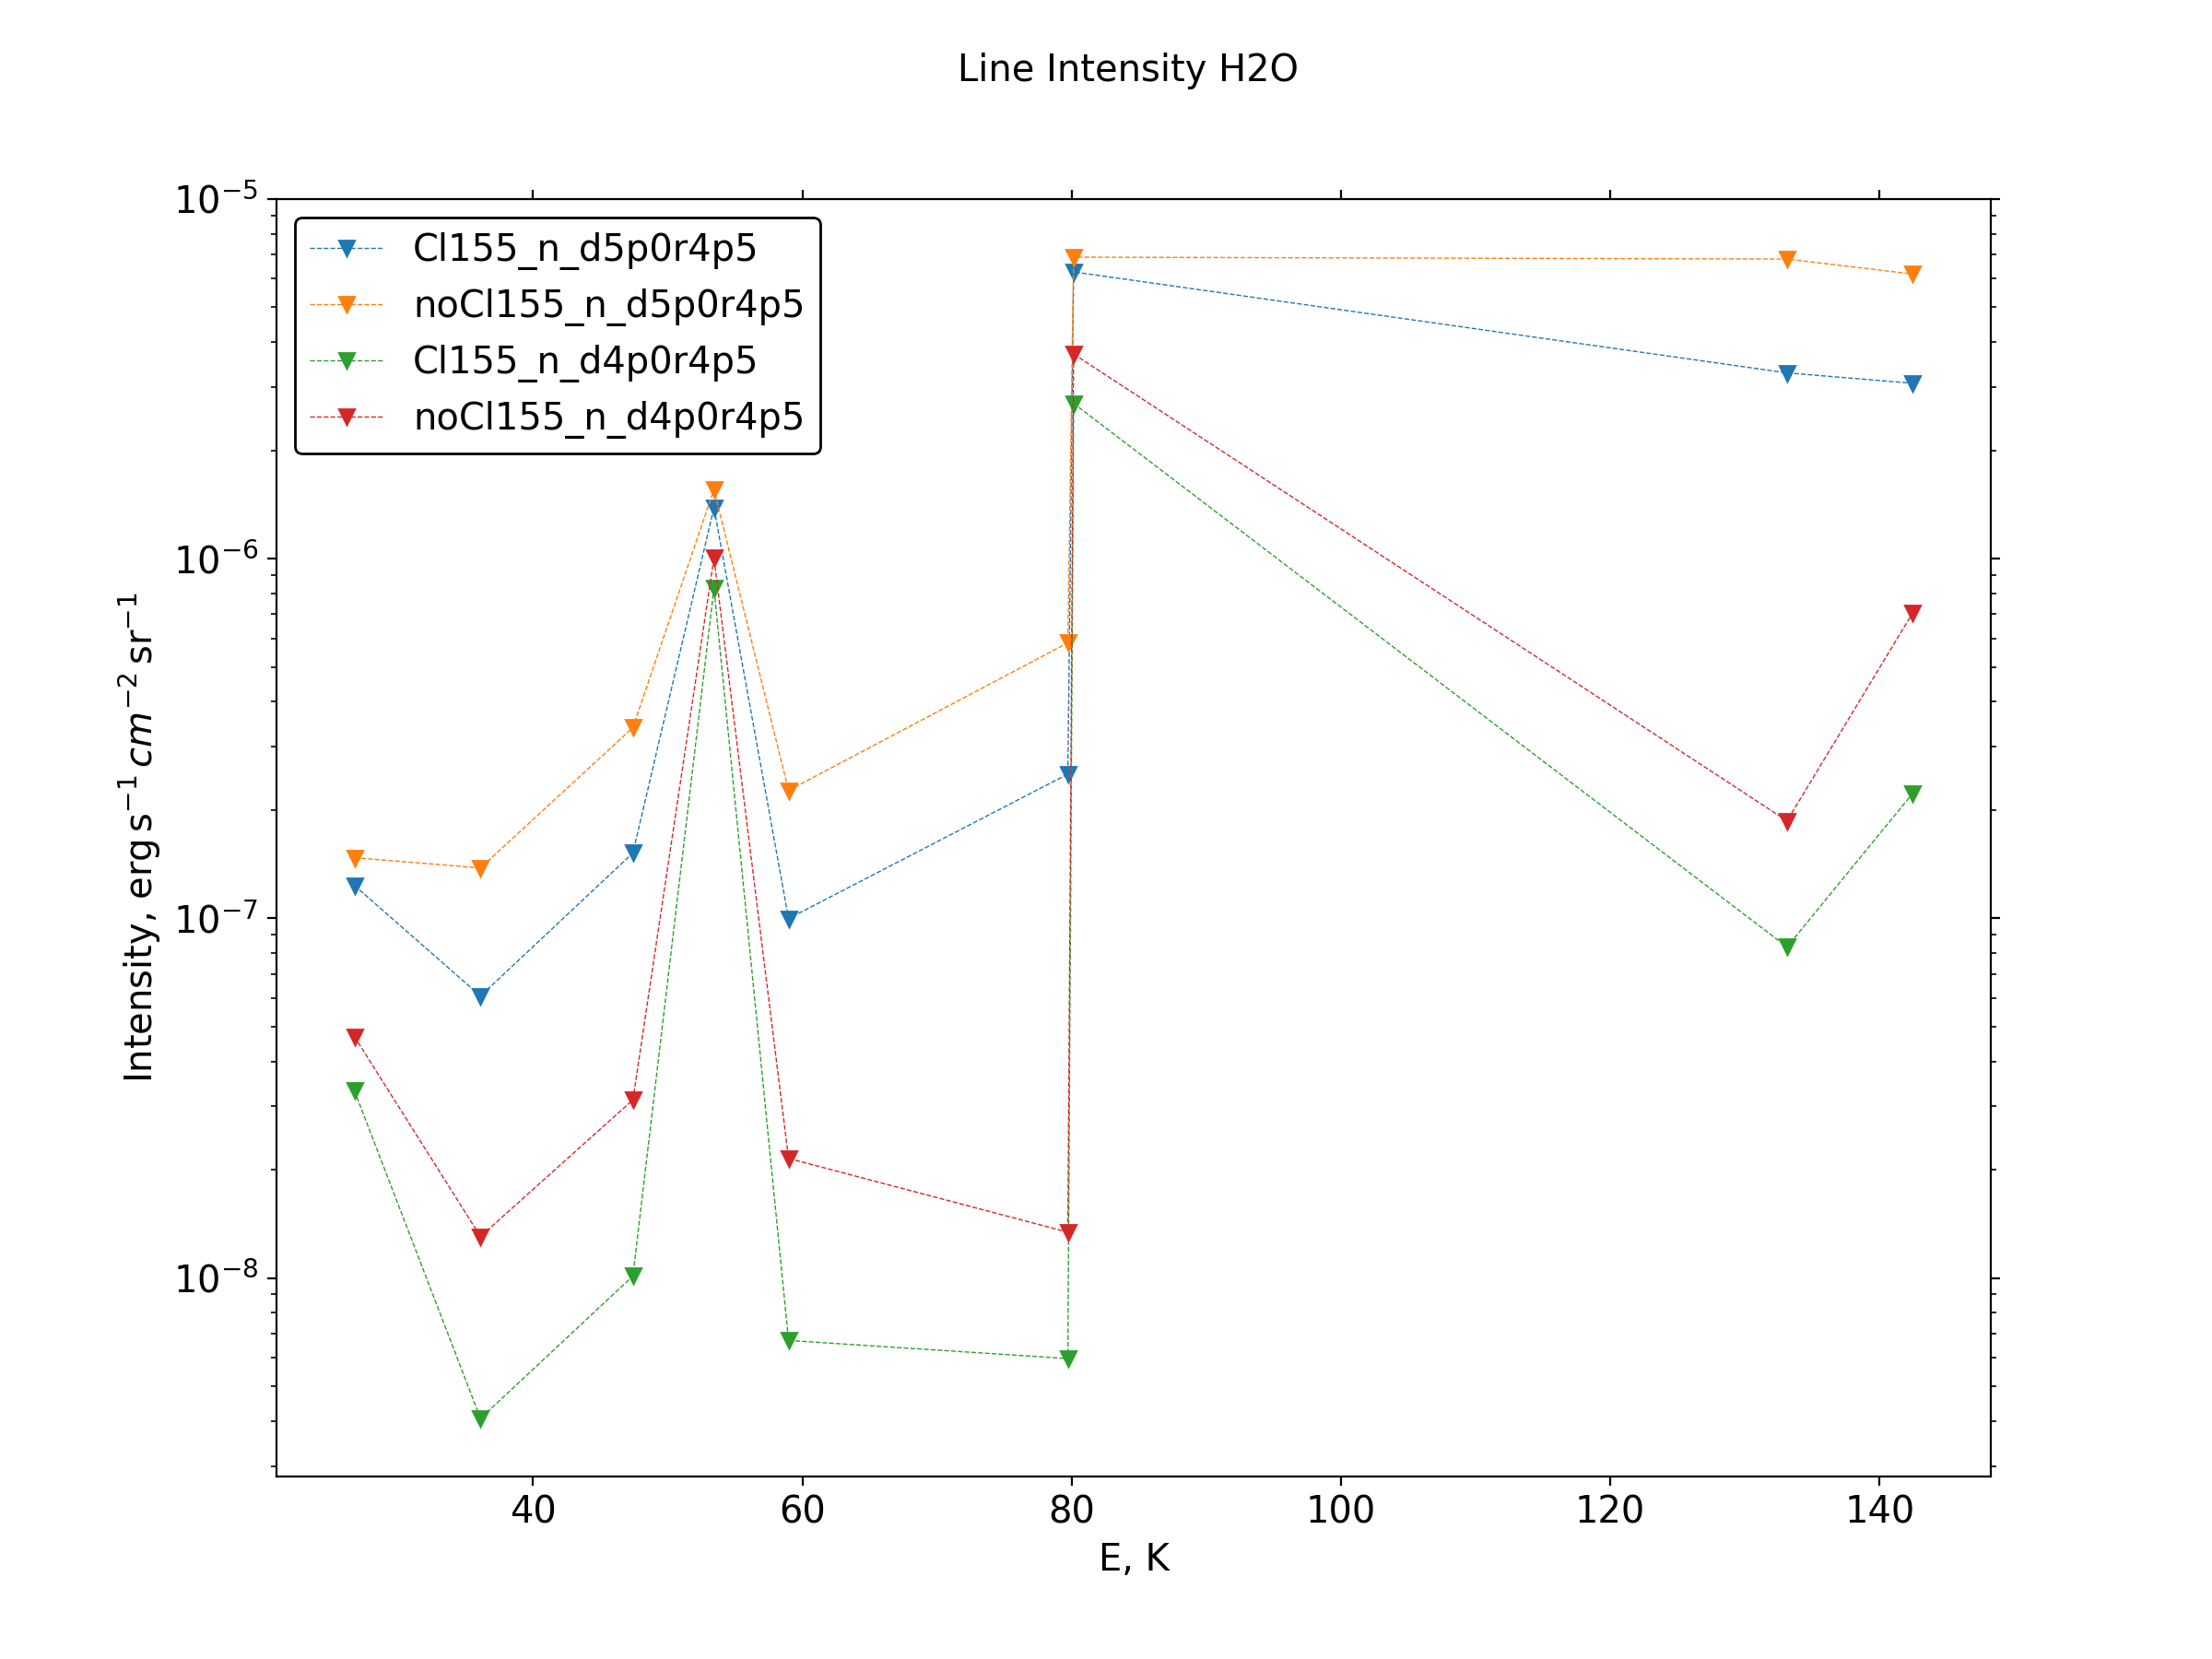
\includegraphics[trim = {0 0 0 1.5cm},clip,width=1\textwidth]{figure/Cl/gridModelEmiss/I_comp_H2O.png}
        \caption{Spectre de $\mathrm{H}_2\mathrm{O}$}
    \end{subfigure}
    
    \begin{subfigure}[t]{0.45\textwidth} % "0.45" donne ici la largeur de l'image
        \centering 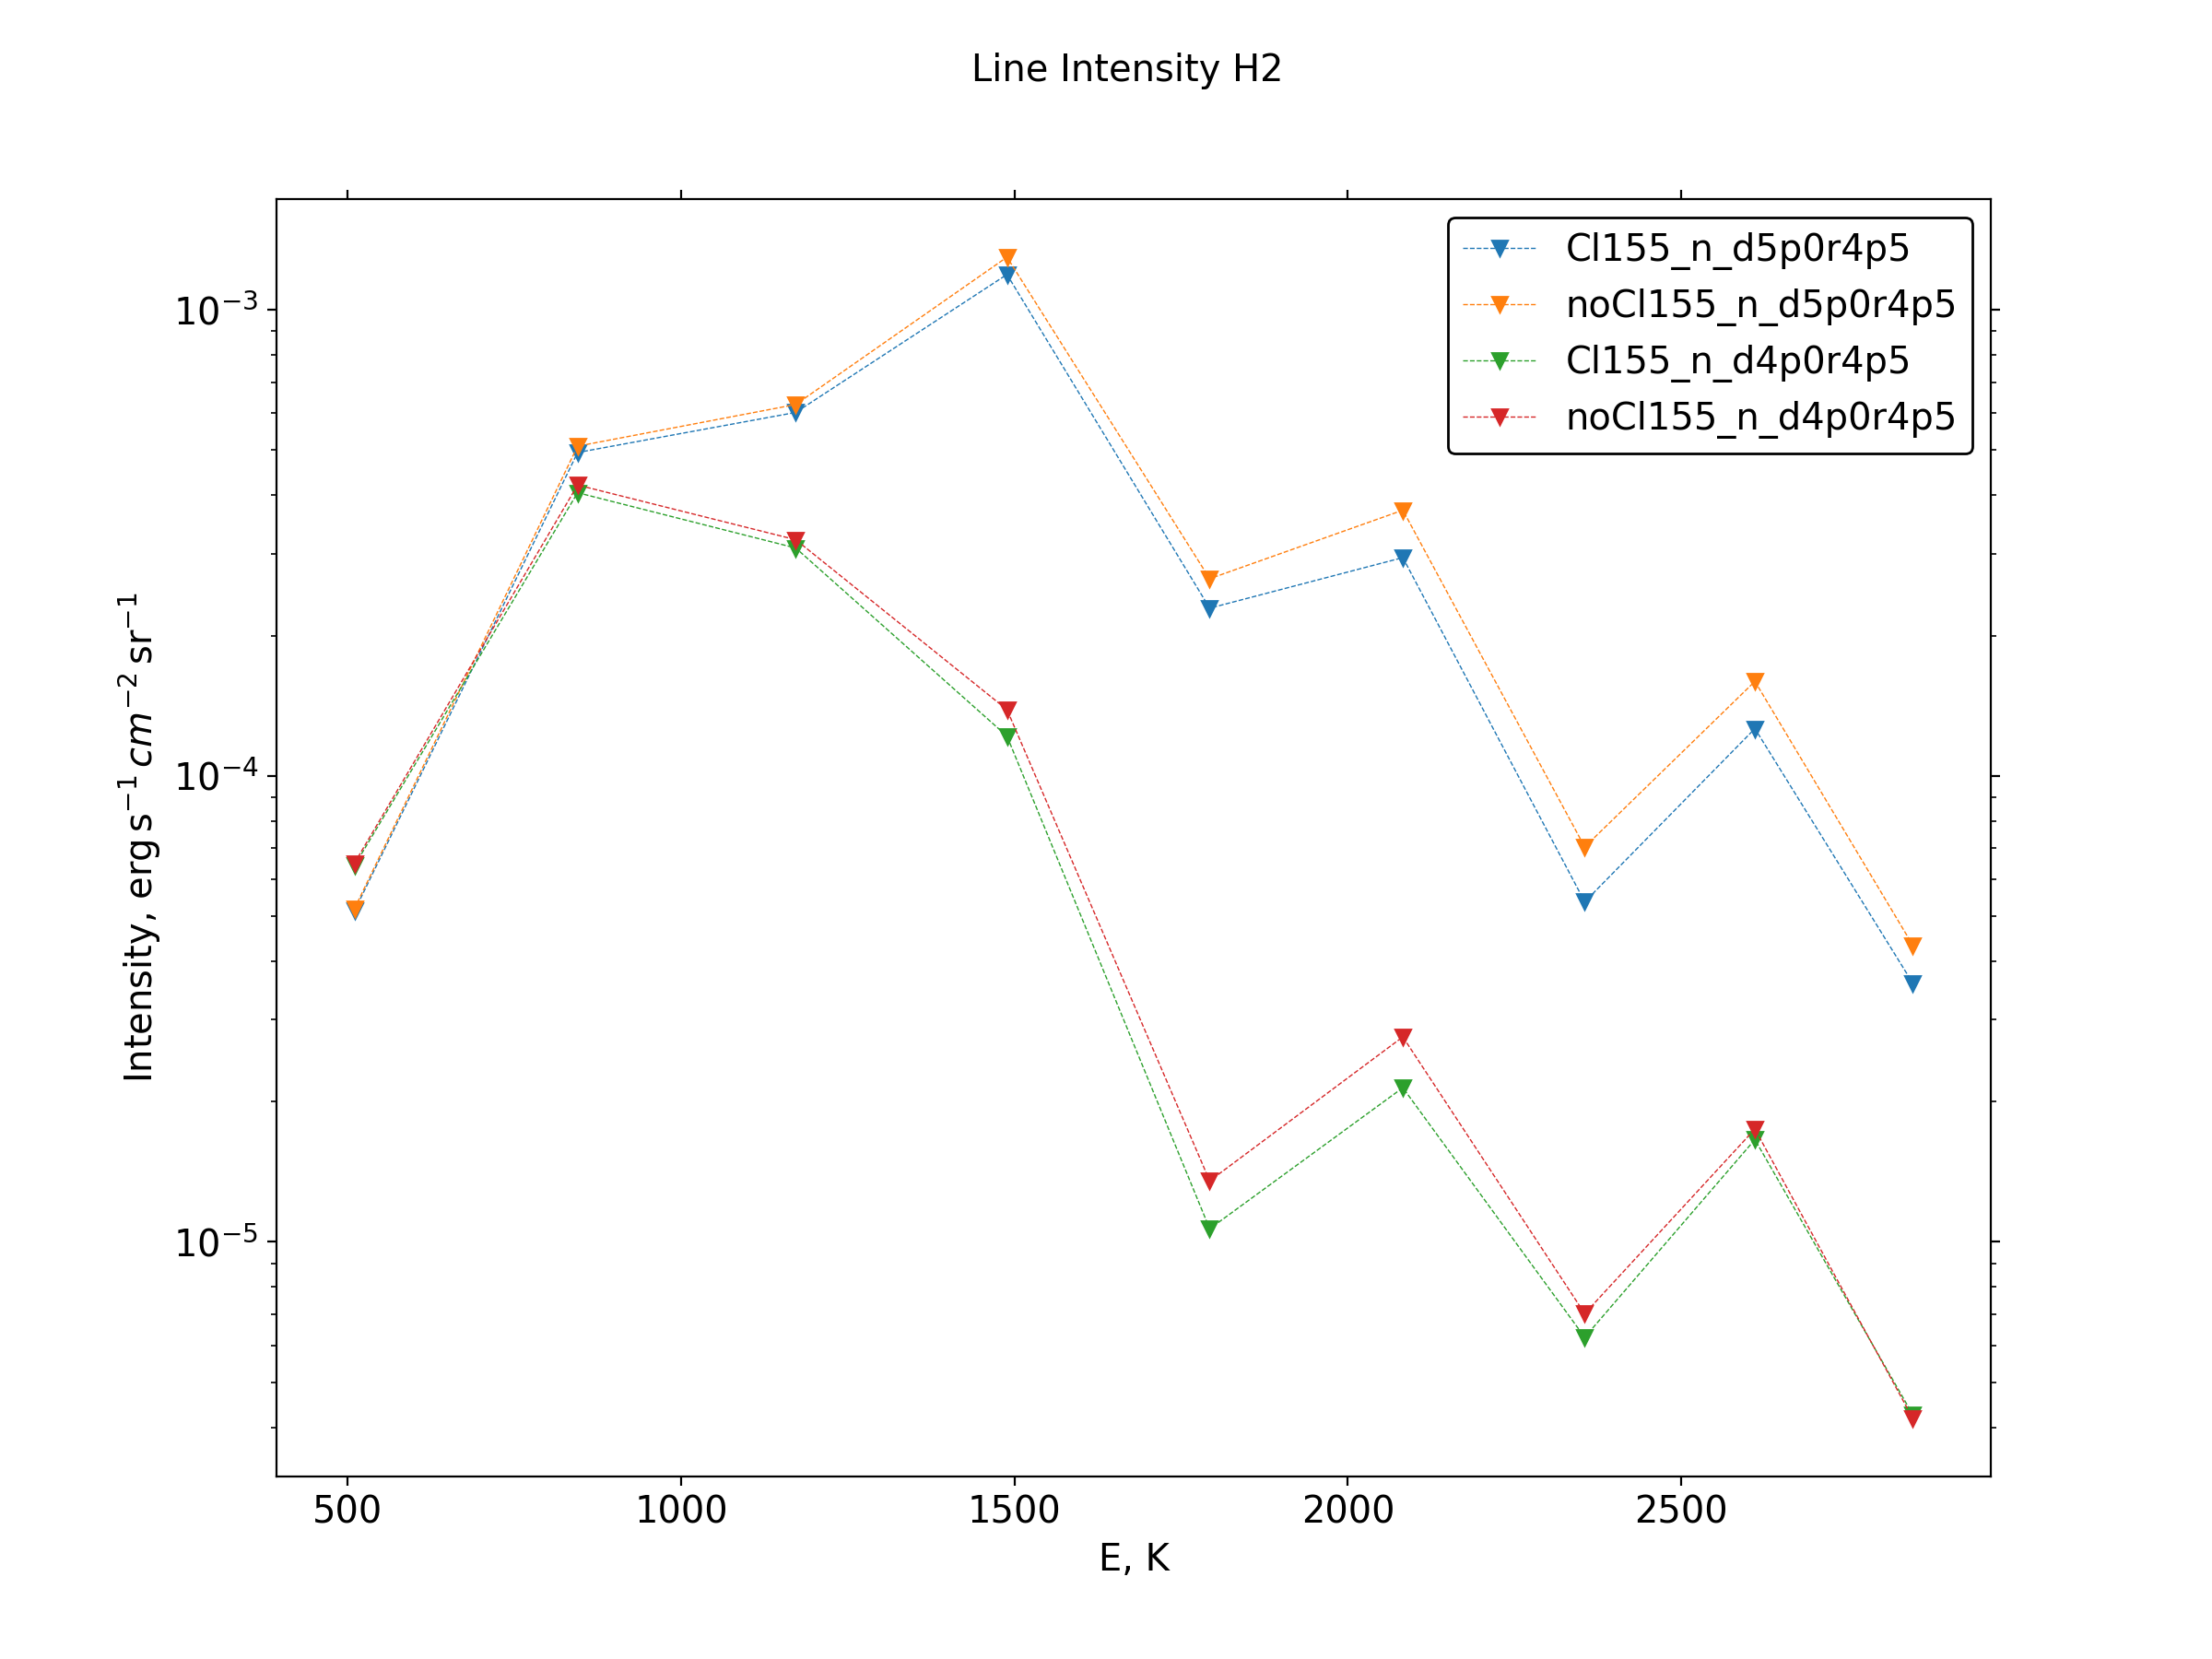
\includegraphics[trim = {0 0 0 1.5cm},clip,width=1\textwidth]{figure/Cl/gridModelEmiss/I_comp_H2.png}
        \caption{Spectre de $\mathrm{H}_2$}
    \end{subfigure}
 
    
    \caption{Spectre chlore code PDR \uncinq}
    \label{fig:Cl:gridModelEmiss:no}
\end{figure}


\subsection{Comparaison de quelques modèles}


%%%%%%%%%%%%%%%%%%%%%%%%%%%%%%%%%%%%%%%%%%%%%%%%%%%%%%%%%%%%%%%%%%%%%%%%%%%%%%%%%%%%%%%%%%%%%%%
